\documentclass{article}

% https://www.cl.cam.ac.uk/local/typography/phd/#margin
\usepackage[a4paper, left=30mm, right=20mm, top=20mm, bottom=20mm]{geometry}

\interfootnotelinepenalty=10000 %% Completely prevent breaking of footnotes

\usepackage{nameref}

% https://ctan.math.illinois.edu/macros/latex/contrib/tkz/pgfornament/doc/ornaments.pdf
\usepackage{pgfornament}

\usepackage{amsmath, amsthm, amssymb}
\usepackage{amsfonts}
\usepackage{mathrsfs}

\usepackage{graphicx} % Required for inserting images

\usepackage{yfonts,color}
\usepackage{lettrine}
\usepackage{marvosym}

\usepackage{hyperref}

% Description list indent
% https://tex.stackexchange.com/questions/9760/indenting-description-lists
\usepackage{enumitem}
\setlist[description]{leftmargin=\parindent,labelindent=\parindent}

% for [H]
% https://www.overleaf.com/learn/latex/Errors/LaTeX_Error%3A_Unknown_float_option_%60H%27
\usepackage{float}

\newcommand{\util}{\scalebox{0.75}{\text{\Pfund}}}

\usepackage[backref=true]{biblatex}
\addbibresource{ref.bib}

\title{{\bf Essay on uncertainty} \\ \pgfornament[height=0.8cm]{84}}
\author{József Konczer\footnote{
\href{mailto:konczer.j@gmail.com}{konczer.j@gmail.com},
\href{https://konczer.github.io/}{konczer.github.io}}
}
\date{December 2024}

\begin{document}

\maketitle

\section*{Opening}


\lettrine[lines=2]{T}{he} subject of this essay might seem hopelessly vast and ungraspable, almost by definition.
However, I do not attempt to discuss uncertainty itself, instead I will examine mainly the possible strategies by which one can cope with uncertain factors.

In general, it is very hard -- perhaps impossible -- to say or suggest anything meaningful or well-founded about the ``unknown''. If we take an honest look at the possibilities in a real-world scenario, then we have to conclude that we have no real good arguments by which we could rule out any shape into which reality might fold out\footnote{Some might feel that I declared the solution to the ``problem of induction'' \cite{sep:Induction} too boldly. Let me try to clarify my statement by taking an imagined ideal casino as an example. I would make the same statement for gamblers playing Hazard or Craps in this casino. I cannot see any good argument that could rule out any result from a throw of a pair of dice. However, not being able to rule something out does not mean that there are no better and worse heuristics for gambling. Furthermore, it does not mean we can not have some advantage at the Blackjack table by, for example, counting cards.
Bertrand Russell wrote the following: ``When one admits that nothing is certain one must, I think, also admit that some things are much more nearly certain than others.'' \cite{book:AtheistOrAgnosticRussell}, by which I absolutely agree on the importance of refining the position, but in my view strategy and action can be regarded more fundamental then believes.

In fact, the primary purpose of this essay is to introduce and discuss such heuristics, hopefully, applicable not only in ideal casinos but also in real-world scenarios.
}.
We might have good heuristics -- such as our own experience, scientific findings, and possibly other guiding principles -- which would be faulty to disregard\footnote{The concept of the impossible, limits, and no-go theorems are useful and fruitful tools of mathematics, science, and engineering \cite{book:Impossibility}. However, these concepts has to be understood in their context and not elevate them -- mainly those which are related to Nature i.e. are not purely mathematical -- to a dogma, because not only futile attempts but sometimes self imposed constraints can also hinder progress. After all, science should not worship what is known but to question it \cite{book:TheAscentOfMan}.}, but in my view, none of these has the power to bring certainty.
(This does not mean, however, that operating in an uncertain world would be impossible. Organisms make decisions and act continually. Realizing that thinking can not bring certainty only emphasizes that acting in the real world is more of an art than a science.)

To overcome this both disturbing and liberating relationship with reality, it is safer to start discussing simpler, idealized decision-making problems for the sake of constructing a theoretical framework.
Although these examples suffer from idealization, they hopefully can function as prototypes, leading to reasonable and useful heuristics.
Adopting a self restrictive definition\footnote{See Von Mises \cite{book:VonMises} for elaborating on ``analytic'' and ``synthetic'' definitions of ``probability'', referring back to Kant. And/or Carnap's explication of the concept of probability in \cite{book:CarnapLogicalFoundationsOfProbability}.} of ``probability'' has been used several times to grapple with the concept.
Games of chance,
%\footnote{See \emph{Philosophical Essay on Probabilities} by Laplace \cite{book:Laplace}.}
repeatable mass phenomena,
%\footnote{See \emph{Probability, statistics, and truth} by Von Mises \cite{book:VonMises}.}
situations where our experience allows us to formulate a degree of belief
%\footnote{See \emph{Probability theory: the logic of science} by Jaynes \cite{book:Jaynes} and \emph{Truth and Probability} by Ramsey \cite{essay:Ramsey}.}
and the case of specific physical systems (such as chaotic/ergodic systems
%\footnote{See \emph{Ergodic Theory} by Sinai, Cornfeld and Fomin \cite{book:ErgodicTheory}.} 
and quantum states)
%\footnote{See \emph{Mathematical Foundations of Quantum Mechanics} by Von Neumann \cite{book:NeumannQuantum}.}) 
have all been used to restrict the domain of uncertainty for the sake of model making\footnote
{
I suggest the following references for the listed approaches (in the same order):
\emph{Philosophical Essay on Probabilities} by Laplace \cite{book:Laplace};
\emph{Probability, statistics, and truth} by Von Mises \cite{book:VonMises};
\emph{Probability theory: the logic of science} by Jaynes \cite{book:Jaynes}, \emph{Truth and Probability} by Ramsey \cite{essay:Ramsey};
\emph{Ergodic Theory} by Sinai, Cornfeld and Fomin \cite{book:ErgodicTheory};
\emph{Mathematical Foundations of Quantum Mechanics} by Von Neumann \cite{book:NeumannQuantum}.
}.

In this essay, I attempt to impose a little less restriction on the concept than in previous works.
Because of the broader scope, the introduced framework can be viewed as the generalization of previous frameworks, even if it is still very far from a general theory of the uncertain.

\section*{Proposed framework}

Probably the best way to introduce the proposed framework, is to clearly list its assumptions, together with the suggested strategy. Let us assume, the followings:

\begin{description}
    \item[0.)] $\star$ There is an ``Agent'' who is part of the ``World''. The Agent can only partially model the whole World, she can develop heuristics, and, most importantly, perform actions;
    \item[1.)] The Agent considers only a finite number of possible actions. The set of actions will be denoted by $\mathcal{A}$;
    \item[2.)] The Agent can (or is willing to) restrict the possible states of the world to a finite set. We will denote this set by $\Theta$ and call it the parameter set;
    \item[3.)] Lastly, the Agent can associate utilities (or rewards) to all potential consequences, which depends both on her action and the state of the world. This function (in the finite case representable by table or a matrix) will be denoted by $U: \mathcal{A} \times \Theta \mapsto \mathbb{R}$.
\end{description}

Under these assumptions, the game-theoretic framework for decision-making and statistics suggests the following strategy for the Agent:

\begin{description}
    \item[I.)] Imagine that the unknown parameter $\theta \in \Theta$ has been chosen by an opponent whose utility function is the regret of the Agent;
    \item[II.)] Determine the Nash equilibrium for such a two-player non-cooperative game: $\langle \sigma^*; \pi^* \rangle$;
    \item[III.)] Adopt the equilibrium strategy $\sigma^*$ of this imagined game to choose an action from the action set $\mathcal{A}$.
\end{description}

The primary goal of the following treatise is to elaborate on this procedure and show the viability of the above-suggested decision-making strategy.


\section*{Objections, defences and remarks}

\paragraph{Whom is this essay addressed to?}
It is a natural question for a reader ``Is this essay for me?'', ``Am I supposed to understand the following?''

The topic of this essay is vast in scope and interdisciplinary by nature.
The institutional walls of today's academia are thick, disciplines often develop separate norms, have their own technical jargon, sometimes similar concepts are independently introduced, and often fields stay in their own confinement and do not refer to literature outside of their abstract intellectual niche\footnote{Although data shows that science becomes more interdisciplinary in the last century \cite{paper:NaturePapersInterdisciplinary,paper:ACenturyOfPhysics,book:AtlasOfKnowledge}, increased specialization can simultaneously happen \cite{paper:BurdenOfKnowledge}, because of the exponential growth of papers and fields alike \cite{book:AcademicTribesAndTerritories}. (The amount of subfields can be illustrated by the number of listed first-level categories in widely used classification schemes. The \href{https://mathscinet.ams.org/mathscinet/msc/msc2020.html}{Mathematics Subject Classification} lists 98 subfields, \href{https://physh.org/browse}{Physics Subject Headings} lists 17 disciplines and the \href{https://dl.acm.org/ccs}{ACM Computing Classification System} lists 13 subfields.)}.
Given these circumstances, scoping has been a hard challenge -- and I am not sure I succeeded.

My solution attempt to this challenge was that I pictured my audience as my younger, less experienced self. A person with some background in probability theory and statistics -- both in theory and practice -- but who was perplexed about its foundations and baffled about the discipline's success against its seemingly ad hoc techniques and foundation.
The aim to write about the topic and embed it into a broader context occurred to me because a similar text would have been very valuable and eye-opening to me a decade ago, before I dared to embark on the quest for recovering -- or constructing -- deeper-lying foundations for probability theory and statistics.

Besides clarifying my own thoughts, I wanted to keep the text intelligible for a broad and diverse audience. The tone and the topics are perhaps more suitable for an academic audience, but hopefully, many aspects are presented in a way that can be appreciated by the general public.
The structure of the essay follows a classical ``dialectic'' philosophical style\footnote{The reason I resorted to wordy philosophical arguments and literary narratives was the lack of already existing formal tools by which I could grasp the relevant aspects of decision making doctrines and reasoning about various heuristics, values and metaphysical constructions. I tried my best to demonstrate the feasibility and computability of the proposed framework for the simplest possible toy model in Statistical Games \cite{arxiv:StatisticalGamesKonczer2024} which is a work mostly about the mathematical \emph{how}. This essay aims to address the philosophical \emph{why} with softer and more delicate philosophical arguments -- mostly using deduction, analogies and abduction -- as an ``epistemic practice'' \cite{sep:Arguments}.} -- with objections and defences --, but the whole text is not moulded into a single coherent narrative. Every objection grasps a different aspect of the problem, some philosophical, some mathematical, some more general. The objections are organized into paragraphs that rarely refer to each other, structuring the text into a loose collection of episodes. Therefore, they can be read separately according to the reader's taste and their own emerging doubts.

\paragraph{Don't we already have a good enough understanding of the topic?}
Haven't statisticians and philosophers already spilt enough ink discussing the foundations and techniques of probability and statistics?
There are authoritative textbooks\footnote{Such as \cite{book:FellerIntroductionToProbabilityV1,book:FellerIntroductionToProbabilityV2,book:Renyi1970,book:Klenke,book:FoundationsOfModernProbability} for probability theory and \cite{book:StatisticalInference,book:CoxStatistics,book:DeGrootProbabilityAndStatistics} and \cite{book:Jaynes,book:Bernardo,book:BoxBayesianInference,book:BayesianDataAnalysis} for statistics.} with a wide variety of techniques; isn't that more than enough to handle uncertainty adequately?

Undoubtedly, there is a vast literature and a rich history\footnote{For relatively concise historical overviews see several Bibliographic notes in \cite{book:CoxStatistics} or Chapter 2: The Historical Context in \cite{book:ProbabilityAndFinanceGame}.} surrounding uncertainty and the concept of probability.
Statistics is a mature field, and it appears to me that most of its techniques have found their niche of applicability.
``Frequentist'' techniques, also known as classical statistics -- developed and popularised among many others by Fisher, Neyman and Pearson -- work well in data-rich environments if stakes are not extremely high. Bayesian techniques -- associating an ``a priori'' probability distribution to unknown parameters -- perform better typically far from asymptotic regimes. (Therefore, these frameworks can be seen both as complementing or rivalling each other.) Even the sometimes seemingly ad hoc techniques are usually tested in practice and kept only those which don't produce undesirable results. Therefore, I do not argue that the current field of statistics is not a valuable repository of useful heuristics. My aim is to search for an organising principle, which can be viewed as a quest for simplicity in thought.

{\it Charting the landscape:}
Writing an overview feels daunting and frightening because I am sure that the sheer volume of the material and the existing diverse viewpoints make it impossible to give a brief summary on which every mentioned major branch would agree. However, daring this impossible task, an oversimplified characterisation of today's mainstream understanding of uncertainty might be given in the following way\footnote{This simplistic description is only a crude overview for those who are not or minimally familiar with statistics and probability theory. For more nuance, see further footnotes, and for a more comprehensive overview, see the cited resources.}:
In practice, we often encounter events that we can not predict with certainty. Contrary to our lack of knowledge, it has been proven useful to not give up entirely our reasoning about such events but try to characterise their behaviour \emph{as if} it would be random, analogous to coin flips and throws of dice. In the time of writing, the dominant way of characterising uncertain events is to associate a probability distribution with the possible outcomes.
There are two main schools of thought for the interpretation of probability itself. The so-called ``frequentist'' approach, which -- strictly speaking -- defines probability only for infinitely repeatable stochastic experiments simply as the ratio of the number of ``desirable events'' divided by the total number of experiments\footnote{Of course, this is a simplistic definition, but even for modern advanced definitions randomness is defined -- strictly speaking -- only for infinite sequences. Historically von Mises introduced ``collectives'' \cite{book:VonMises} as the models of random sequences (also known as Mises–Wald–Church random sequences). Jean Ville in 1939 proved \cite{book:ProbabilityAndFinanceGame,thesis:Ville1939} that this definition allows sequences which do not satisfy the iterated logarithm theorem, i.e. their ratios don't fluctuate the limiting probabilities but converge from below (or above). This led to more advanced definitions of randomness, such as a construction by Martin-Löf \cite{book:KnuthVol2,paper:MartinLof1966}.}. The so-called Bayesian approach understands probability mostly as a ``degree of belief'' and -- strictly speaking -- prescribes only a rule -- Bayes' rule -- to update one's beliefs in the light of new evidence (therefore, the Bayesian framework in its simplest form stays silent about the initial degree of belief, i.e. the prior probabilities)\footnote{Naturally, the real landscape of Bayesianism is more diverse (I. J. Good mentioned $46656$ different interpretations in \cite{book:GoodThinking}). Two big camps can be identified based on their approach to the question of priors. Subjective Bayesians -- most notably represented by de Finetti \cite{book:deFinetti} -- view priors as a completely subjective degree of belief of an experimenter, while objective Bayesians \cite{book:ObjectiveBayesianInference} tend to seek additional principles -- such as maximum entropy \cite{book:Jaynes,paper:GameTheoryMaximumEntropyGrunwald2004}, invariance under symmetry transformation groups leading to Haar prior(s) \cite{book:Jaynes,book:ObjectiveBayesianInference}, reparametrisation invariance leading to Jeffreys prior \cite{paper:JeffreysPriorOriginal}, maximal ``uninformativeness'' (causing the biggest expected surprise) leading to the reference prior \cite{book:Bernardo} -- to construct ``objective'' or ``uninformative'' priors. (A whole catalogue of uninformative priors has been collected here \cite{misc:PriorCatalog}.)}.

There were times when people -- mostly economists in the beginning of XX. century -- contemplated uncertainties which can not be characterised by probabilities\footnote{See Knight \cite{book:Knight}, Keynes \cite{book:TreatiseOnProbability} and a historical summary of the concept's development in economics in \cite{book:JuliaUncertainty}}.
There was a suspicion that the ``frequentist'' and the Bayesian interpretation might describe related but different concepts\footnote{Such as ``degree of confirmation'', i.e. credence or degree of belief and ``relative frequency in the long run'', i.e. chance \cite{sep:Carnap,book:CarnapLogicalFoundationsOfProbability}.}.
However, seemingly, most contemporary researchers and practitioners operate in a conceptual framework where it is assumed that uncertainty is adequately describable by probabilities, and its objective description is related to the ``frequentist'' interpretation while its subjective description is related to the Bayesian framework.

Statistical techniques stemming from the ``frequentist'' interpretation are concerned with asymptotic properties of a test or a method -- therefore, these are most naturally applicable in data-rich environments i.e. in the ``asymptotic regime''\footnote{For reference see \cite{book:AsymptoticStatistics}.}.
Meanwhile, for Bayesian techniques, the biggest challenge has been the tractability of their method. The emerging popularity of Bayesian techniques can be partially explained by the development of effective numerical methods such as Markov Chain Monte Carlo sampling, by which the required high dimensional integrals become numerically tractable\footnote{For a brief historical overview how this numerical method coupled with increasing computing power revolutionised and generated renewed interest in Bayesian methods in the late 1980s and early 1990s see \cite{paper:ShortHistoryOfMCMC}.}. However, as data gets sparser, the choice of priors becomes more and more important in Bayesian methods, requiring additional principles or heuristics to yield results.

Of course, the real history and the more detailed landscape are much more complicated:
The whole mathematical discipline of probability theory was introduced as an epistemic description, partially founded by Laplace in about 1820, coining the term ``the principle of insufficient reason''\footnote{See Laplace's famous essay at \cite{book:Laplace}. For early European history of probability, see \cite{book:Todhunter1865History}, which is itself a historical specimen -- from 1865 -- reflecting the norms and views of its age. Another book investigating the evolution of concepts related to probability from ancient times to the Newtonian era is \cite{book:GamesGodsGambling}. The three books of Anders Hald cover the topic from antiquity to 1935 \cite{book:HaldHistoryProbabilityStatisticsBefore1750,book:HaldHistoryOfMathematicalStatistics1750-1930,book:HaldHistoryOfInference1713–1935}. For more recent developments see the historical parts in \cite{book:ProbabilityAndFinanceGame} and the Bibliographical notes in \cite{book:CoxStatistics}. For very recent highlights, see a presentation by Yuval Peres \cite{talk:HighlightsFromTheHistoryOfProbability} stretching from Hilbert's 6th problem in 1900 \cite{paper:HilbertProblems1900} to 2024. About the transmission of the concepts of probability theory to other mathematical traditions -- such as China -- see \cite{paper:TransmissionOfProbabilityTheoryIntoChina, book:GlobalHistoryOfMathematics}.}.
The mathematical axiomatisation of probability theory happened relatively early in 1933 by Andrey Kolmogorov\footnote{However, Kolmogorov's mathematical formalisation \cite{book:Kolmogorov} is purely a formal theory: ``Every axiomatic (abstract) theory admits, as is well known, of an unlimited number of concrete interpretations besides those from which it was derived. Thus we find applications in fields of science which have no relation to the concepts of random event and of probability in the precise meaning of these words.'' As such, it is not closely ``tied'' to any interpretation of probability \cite{sep:InterpretationsOfProbability}. Besides Kolmogorov's construction -- which is still the most influential -- other axiomatisations exist. To mention a few alternatives there is Dempster–Shafer theory \cite{paper:Dempster1967,book:ShaferTheoryOfEvidence} (closely related to imprecise probabilities \cite{paper:IntervalProbability,book:UncertaintyInEngineering} and the theory of capacities \cite{book:TheoryOfRandomSets,book:TheoryOfCapacities}), logical probabilities built on Cox's theorem \cite{paper:Cox1946,book:Jaynes,arxiv:Cox} (often derived only for finitely additive measures). For a collection and comparison of several formal approaches, see \cite{book:TheoriesOfProbability}.}. It provided a rigorous formal framework built on measure theory in which theorems could have been stated, and it provided tools that proved fertile in other branches of mathematics\footnote{For probabilistic techniques in graph theory, number theory and more see \cite{book:TheProbabilisticMethod,book:ProofsFromTHEBOOK}.}. 
There was a temporary enthusiasm in the 1950s regarding -- non-Bayesian -- statistical decision theory, mostly related to Abraham Wald and his book\footnote{Where Wald introduces a zero-sum game between the ``Experimenter'' and ``Nature'' and defines equilibrium strategies for such a fictional game. The book is rather technical but had a considerable impact \cite{book:Wald}. Savage summarised, modified and criticised Wald's construction and introduced half-heartedly the concept of minimax regret in \cite{book:Savage}. (Jürg Niehans proposed independently a deterministic minimax regret decision rule regarding economic pricing in 1948 \cite{paper:MinimaxRegretNiehans1948}.)} in 1950:
``This work lead to the view, widely held for a period, that all statistical
problems should be formulated in terms of decision making.''\footnote{Quotation from the Bibliographical notes of chapter 11 Decision theory in \cite{book:CoxStatistics}.}.
Today, quantum systems are characterised by another kind of non-commutative algebra of observables, replacing probabilistic density functions with density matrices\footnote{Quantum mechanics \cite{book:NeumannQuantum,book:WeinbergQuantumMechanics} and quantum logic \cite{paper:NeumannBirkhoffQuantumLogic} is itself an immense field. On a surface level, two related interesting phenomena should be mentioned if contrasted with classical probabilistic descriptions. Entanglement -- causing ``extra correlations''\cite{book:PitowskyQuantum} -- and non-commutativity which forces to change the structure of events or observables from a commutative lattice (representable by a collection of subsets in classical probability theory) to an ``orthomodular lattice''\cite{sep:QuantumProbability,arxiv:Pitowsky,book:AxiomsForLattices} (representable by linear projections on a vector space with scalar product i.e. projectors on a Hilbert space). These special features of quantum systems, such as superposition and entanglement, made it possible to develop new computing technologies such as quantum computing and quantum information theory \cite{book:QuantumComputationAndInformation}.}.
Work has been done in algorithmic probability theory, which by associating a universal prior to discrete -- or rather digital -- patterns related to their complexity\footnote{For further resources see \cite{book:LiVitanyi,book:Solomonoff,book:UniversalArtificialIntelligence}.}, can provide a rich framework and be used for inference in theory (and simplified versions in practice). In my view, this is a fascinating direction as well, but seems to fall outside of today's mainstream.

{\it Positioning the proposed framework:}
Relative to this landscape, the proposed framework can be viewed as the continuation of statistical -- or robust\footnote{See \cite{book:RobustnessAnalysis} for the connection between Wald's minimax principle and robust decision theory. To see relations with robust control, see \cite{book:Control,book:RobustAndOptimalControl}.} -- decision theory -- more particularly approaches related to minimax regret -- which was popular in the 1950s, but fell out of the mainstream at about 1960s\footnote{``In the late 1950s and early 1960s theoretical interest shifted from the situation without prior distributions to Bayesian decision theory in which personalistic prior distributions and utilities are central to the argument'' \cite{book:CoxStatistics}.}. It is, therefore, applicable to uncertain parameters that are not well characterisable by a probability distribution (described by Knight and Keynes in the first part of the XX. century).

The framework restricts itself to ``known unknowns'' first and doesn't address immediately the ``unknown unknowns''\footnote {As Donald Rumsfeld famously declared: ``There are known knowns; there are things that we know that we know. We also know there are known unknowns; that is to say, we know there are some things we do not know. But there are also unknown unknowns, the ones we don’t know we don’t know.'' \cite{book:WhatWeCannotKnow,book:RadicalUncertainty,book:TheBlackSwan}.}. However, it has a natural continuation to ``describable unknowns'' which could be potential events not coming from a finite set of possibilities, but any event which can be described with a string of characters e.g. described by written language\footnote{A relatively simple construction can yield an equilibrium strategy eerily similar to Solomonoff's induction formula \cite{book:Solomonoff}.}.

{\it Justification of the effort:}
To address the original objection, this project's modest goal is to revitalise and repopularise the concept of uncertainty and statistical decision theory framework in light of new concepts and applications.

The more ambitious goal of the project is to embed the diverse and numerous collection of techniques in statistics into one coherent, unified framework, in which the seemingly separate approaches can be understood as different limiting cases or as decision-making tools for various objectives.


\subsection*{Discussion of the assumptions}

As we now delve into the proposed framework, I should first discuss the assumptions it requires.

\paragraph{Separating the Agent from the World:}
How is it possible for the Agent to maintain a separate identity from the World? How do the Agent's preferences come to be? What does it mean to ``choose'' for the Agent?

In my view, these are all valid questions\footnote{
Most philosophical and religious frameworks assume or recognise a concept of ``self'' \cite{sep:Identity,book:WorldsReligions,book:FunfWeltreligionen} as a separate -- or at least not identical -- entity with the ``World''.
(Several mystical branches arrive at a view of Unity (or non-duality). However, these frameworks are often considered as advanced -- and often controversial -- teachings that are not comprehensible or suitable for everybody or in every stage of life or role in society. A few related concepts might include: Nature as the one substance by Spinoza \cite{book:SpinozaEthics, sep:SpinozaPhysics}, Godhead by Meister Eckhart \cite{book:RoyceEckhart,sep:Eckhart,book:Eckhart}, Wahdat al-Wujud often attributed to Ibn 'Arabi \cite{sep:IbnArabi,book:HistoryOfIslamicPhilosophy,book:IbnArabi}, Advaita Vedanta by Shankara \cite{sep:Shankara,book:AdvaitaVedanta}, Sunyavada by Nagarjuna \cite{sep:Nagarjuna,book:Nagarjuna}, etc.)

Even without believing in the independent, True existence of an individual ``self'' or agency, one can still find such a framework useful merely as an effective theory.
%Although one does not need to believe in the independent True existence of an individual ``self'' and agency to find a framework assuming these useful, merely as an effective theory. 
I see the game-theoretic framework as a favourable plateau from which we can have a better view and which offers a more robust and more consistent framework before continuing our journey of understanding.
For a possible path where individuals emerge -- instead of being postulated --, see, for example, the paper of Krakauer et al. \emph{The information theory of individuality}  \cite{paper:Individuality}.

This framework aims to help navigate the uncertain world for those who are -- or at least play the role of being -- in the state of separation. However, I hope that suggesting strategies in imagined games will contribute more to enhance the overall conditions for enjoying the play, then solidifying the illusion of the game itself.

I think we can stay just as perplexed about the intricacies of the ``self'' (or Agents in our context) as Isaac Newton was on ``causes hitherto unknown'' \cite{book:Principia, book:Principia1848, sep:Principia} for action at a distance in his law of universal gravitation \cite{book:CorrespondenceOfIsaacNewton,paper:NewtonOnActionAtADistance}; unless a framework assuming individuals can go near the fruitfulness of the success of the inverse square law in celestial mechanics. By not excluding the possibility of further generalisation and reinterpretation of the theory as emergent, this assumption hopefully does not prevent deeper understanding in the future.
}
, but in this essay, I will not attempt to clarify or investigate the emergence or the workings of the willing, thinking and acting faculties of the Agent from the ``Naturalistic perspective''. I will assume that such an Agent or Organism is given -- or at least that this description can characterise some existing structures well. If I am honest, I need to admit that this is an idealisation, hopefully a useful one.

\paragraph{Where are the preferences coming from?} In this framework, it is assumed that the Agent \emph{has} preferences. Moreover, we assume that these preferences are characterizable by a utility function. To address the question, preferences may stem from or be shaped by various sources. For humans, they might arise from evolutionary pressures, cultural influences, psychological tendencies or conditioning, or any mixture of mentioned or further factors.

This framework can be viewed as a goal-agnostic way of addressing uncertainty in decision-making situations. This might signal that it aims to be ``only'' an effective theory. Still, I think this is a safer, pragmatic way to construct a framework that does not take firm ideological positions prematurely and can be refined by acceptable preferences separately. Finding and formalizing what ``acceptable preferences'' might mean seems to be a delicate matter,  which is extremely important. However, because it can not get the deserved care and depth here, it has to be 
outside the scope of this essay.
I can only hope that those who apply this theory, will adopt -- by choosing or inheriting -- their values and preferences wisely.

\paragraph{Possibilities without probabilities:}
Some might question the third assumption, or more precisely, the lack of – subjective – prior probabilities associated with the possible states of the world: $\Theta$. 

This objection\footnote{Maybe closest to the subjective Bayesian position \cite{sep:BayesianEpistemology}, most famously advocated by Bruno de Finetti \cite{book:deFinetti}.} is not easy to answer completely, but it seems to me that there are good arguments for why an Agent should have decision-making processes in her repertoire for cases when no prior is justified.
I agree that if the Agent has plentiful credible experience or information about the possible states of the world, this should be incorporated and then continue with standard (for instance, Bayesian) decision-making process.
However, I disagree with the suggestion that model-making always requires (or implies) a conditional prior, given all knowledge the Agent has. In the light of a more general framework, requiring a prior might seem like forcing the Agent to pick unfounded beliefs prematurely.

{\it Insights from black-and-white thinking:}
Giving a definitive counter-example that shows the absurdity of requiring a prior from the Agent seems impossible to me. I could list more or less convincing examples, such as decision problems on other planets, in constructed virtual worlds, predicting the results of future physical experiments, which are outside of the domain of validity of successful present theories; but ultimately, none of these examples seems unobjectionable for me.
Instead of searching and constructing more elaborate examples, I aim to show that even a Bayesian can not convince only by a simple counter-example, an Agent who is committed to black-and-white thinking.

Perhaps this more extreme requirement can illustrate how premature judgements can cause ``hard to accept'' decisions:
Imagine that a ``subjective logicist'' believes that all propositions must ultimately be either true or false\footnote{Also known as ``Dichotomous Thinking'' in psychology \cite{book:DichotomousCBT}.}. Therefore, model-making requires picking a definite non-contradicting set of truth values for propositions, i.e. believing and choosing one definite state from $\Theta$.
This might look like an extreme requirement and can lead to an extreme decision-making process, but formally, it seems just as hard to rule out as demanding a subjective prior\footnote{
One might think that whenever a ``subjective logicist's'' firm belief turns out to be false, she might need to give up her decision-making doctrine.
However, she can simply admit that she has chosen the wrong axioms, which turned out to be inconsistent with the facts, but then she picks another non-excluded set of axioms, i.e. she can continue following her black-and-white decision-making process.
This shows that the ``subjective logicist'' is not incapable of learning from experience, and this partial flexibility makes it harder to challenge her doctrine.
}. Agents who follow a ``subjective logicist'' doctrine can sometimes win, and if they guess the state of the world correctly, they may be more successful than more cautious players.
This example shows that even in extreme cases, there are no obvious arguments by which one could definitely rule out an Agent's decision-making doctrine.

However, there are weaker arguments:
\begin{itemize}
    \item The ``subjective logicist'' framework can be reinterpreted as a particular case of a subjective Bayesian framework because if the Agent has very strong background knowledge, then her prior can be concentrated on one single state from $\Theta$, and her choice of action become indistinguishable from a ``subjective logicist's'' behaviour (if both happened to believe in the same state).
    \item There might be situations where the doctrine of a ``subjective logicist'' ``feels'' extreme, and the definite choice of a state forced and premature.
\end{itemize}

I do not see much better arguments for considering a framework which does not demand the Agent to develop a prior for the possible states. One can show that in a multi-level game setting, as the amount of collected data from other rounds goes to infinity, the collected data can be incorporated into further decision-making as a prior, i.e. the Bayesian framework can be interpreted as a particular limiting case of the game-theoretic framework. Further, one can ``feel'' that there are some decision-making problems in which no specific prior is well founded, and a prior choice would seem forced and premature.

% O: Sometimes we want to have continuum spaces
% D: The model starts with finite, which is an advantige relative to jefries + reference priors, then continuum spaces can be reahed by taking the limit. There are somewhat pathological cointeraxmples, where equilibrium does not exist, but in most cases that is fine.
\paragraph{Finiteness:}
An objection against both the second and third assumptions about the finiteness of the sets of states and actions is that, sometimes, they are better modelled by continuous quantities. As a result, a finite framework might seem inadequate in such cases.

The main defense to this objection is that continuous models can be defined as appropriate limits of finite models. Being able to address discrete models can be viewed as an advantage of the framework compared to some ``objective Bayesian'' frameworks, such as parameterization invariant priors\footnote{Also known as Jeffreys prior \cite{book:Jaynes,paper:JeffreysPriorOriginal}.} which can be defined naturally on continuous parameter sets.

Of course, reaching a continuum limit from finite quantities can open new questions of convergence. There are general theorems guaranteeing the existence of a Nash equilibrium for continuous games\footnote{See for example \cite{paper:ContinuousEquilibrium,paper:SeparableGames} for reference.}, but there are examples of discontinuous continuum games with no equilibrium solution\footnote{See ``the game without value'' as an example \cite{paper:DiscontinuousGames}.}.
However, naturally occurring examples seem to have well-behaving continuum limit\footnote{To see how game-theoretic equilibrium calculations can be performed on continuous spaces, I suggest reading the following papers \cite{Kashyap1971,Kashyap1974,paper:Abbott2018,paper:Abbott2023}.} (even if the requirements of the general theorems on continuous games are not satisfied, usually one can find unique equilibrium points by direct calculation).
Perhaps it is possible to construct pathological examples, but this can also be done in standard probability theory\footnote{To see a collection of counterexamples see \cite{book:CounterexamplesInProbability,book:CounterexamplesInProbabilityAndRealAnalysis,book:CounterexamplesInProbabilityAndStatistics}.}.
Exploring the sufficient requirements for a well-defined continuum model remains a task for future mathematical investigations, but it seems like a reachable goal which can be achieved gradually, just as probability theory as a mathematical discipline based on measure theory has been established and then further generalized to stochastic processes.


%An obvious objection against both the second and third assumption about the finiteness of the sets of states and actions is naturally valid, but discriminating ``important'' (or ``relevant'') possibilities and actions from all imaginable (or possible) states and actions is an essential task of model making, even if the model will suffer from these idealized simplifications.

%Finiteness can be relaxed\footnote{To see how game-theoretic equilibrium calculations can be performed on continuous spaces, I suggest to read the following papers \cite{Kashyap1971,Kashyap1974,paper:Abbott2018,paper:Abbott2023}.}. One can generalize the framework to a countable infinite or even continuum set of states and/or actions as limiting cases of the finite case.

\paragraph{Assigning utilities:}
%The introduction of the concept of utility and the requirement that the Agent has to be able to associate her own subjective utility with all possible outcomes in the fourth assumption might seem like an additional concept to statistics and a heavy burden put on the Agent.
Introducing the concept of utility, and requiring the Agent to assign subjective utility to all possible outcomes, might seem like an added complication to statistics and a significant burden for the Agent.

However, the concept of utility is essential in most other decision-making processes\footnote{Modern decision theory is concerned with ``goal-directed behaviour in the presence of options'' \cite{paper:DecisionTheoryAnOverview}.}, aided by statistics and/or probability theory. The standard assumption is that a ``rational'' Agent maximizes her Expected Utility\footnote{More on Expected Utility theory see \cite{plato:ExpectedUtility}.}, where the expectation is taken with respect to probabilities determined by statistics and/or a probabilistic/stochastic model. 
%The decision-making process is usually performed modularly: Stochastic models – often aided by statistics – produce probabilities for the possible states, independent of the utilities of the outcomes; then, for all actions, the expected utilities are determined as the weighted sum of outcome utilities; finally, the action providing the maximal expected utility is selected.
The decision-making process is typically modular. First, stochastic models, often supported by statistics, generate probabilities for possible states independent of the outcomes' utilities. Next, expected utilities are calculated as the weighted sum of the outcome utilities for all actions. Finally, the action with the highest expected utility is chosen.


To use probability and statistics for decision-making, one must determine the utility of possible outcomes. The reason why these concepts can decouple is the form of Expected Utility, which is defined as the simple bilinear expression of the probabilities and utilities ($\mathrm{EU}(a)=\sum_\theta U(a;\theta) \cdot \pi(\theta)$).

The main difference compared to traditional frameworks is that in the game-theoretic framework, the main focus is on the actions and strategies, not beliefs or asymptotic frequencies.
In traditional frameworks, the estimation or calculation of beliefs and utilities can be decoupled, while in the game-theoretic framework, the whole decision-making process is interpreted as one unified strategy.

\subsection*{Discussion of the suggested strategy}

After discussing the assumptions, we can take a closer look at the suggested decision-making process.

\paragraph{Imaginary opponent:}
Imagining that the unknown states are chosen by a strategic player is perhaps the most controversial part of the suggested strategy. It might seem like an unfounded metaphysical claim or a form of animism\footnote{Animism is not meant to be a derogatory term here. Animistic belief systems assumes independent personality and motives to non-human beings \cite{book:Animism}, while in the proposed framework the ``motives'' of the unknown depends only on the Agent's preferences.}. 

However, this imaginary opponent is not something the Agent has to wholeheartedly believe or accept. It is only a metaphor, an analogy, which can be adopted—not because of any claim about the unknown, but because such construction can provide ``reasonable'' and generalizable strategies.

To put this aspect into perspective, it is good to notice that no other frameworks are free of metaphysical claims and constructions either.
The classical theory of probability postulates that all possibilities have to be assigned with the same degree of belief -- known as the principle of insufficient reason -- and often introduces idealized devices of chance (such as coins and dice), which are embodiments of stochastic behaviour. (While the associated probabilities are often determined by symmetry arguments.)
In the frequentist framework, it is often postulated that some experiments have inherently stochastic behaviour and that no pattern can be found in their outcomes. The possibility of infinite repetition, the assumption of independence, and the convergence of frequency ratios are all further very strong claims and assumptions appearing in this framework.
In the Bayesian framework, the concept of prior has an unspecified interpretation and might be viewed as a non-strictly empirical component of the theory.

\paragraph{Potential values of science:}
Why can’t we rely solely on objective scientific methods to determine truth and then use that knowledge to guide us in the best possible direction?

The scientific worldview favours objective formulations of ``natural laws'' and ``natural phenomena'' that are not biased by the observer’s beliefs or values. Deducing patterns and principles that are not subservient to popular ideologies has been a very successful project in various fields of science, but science alone can not advise Agents how to act.
In my view, the practical application of scientific knowledge necessitates the incorporation of personal values; therefore, a purely scientific, value-free decision-making process is hardly imaginable.

Moreover, to a large extent, science is an empirical discipline that relies on real-world data to construct models or match parameters. Statistics is the bridge, which is used to connect the finite amount of observation with abstract values, by separating the ``noise'' from the ``phenomena''. Because of this unique position, connecting the complex and mysterious real world with the constructed abstractions of the scientist, a framework of statistics and probability might be judged differently than abstract scientific theories. (Simply put, if we need statistics to test scientific theories, then how could we test statistics itself?) Therefore, it could be acceptable -- or even be necessary -- that such frameworks contain metaphysical elements, including values or utilities. 

However, it might be possible to keep the scientific project separate from subjective values and ideologies if we spell out scientific values. A natural scientific value might be a form of simplicity (quantitatively the length in bits of the model and the data\footnote{This is the core idea of the Minimum Description Length (MDL) principle \cite{paper:MinimumDescriptionLengthRevisited,book:MinimumDescriptionLength}.}), predictive power (the success rate of guessing the outcome of not yet performed experiments\footnote{This aim coupled with algorithmic probability \cite{book:LiVitanyi} can lead to the Solomonoff induction formula \cite{book:Solomonoff,book:UniversalArtificialIntelligence}.}), and possibly other information-related measures. In this way, science does not need to maintain that it is value-free, but it has to spell out its ideology-free ``neutral'' or ``scientific'' values.

A family of ``natural'' utility functions has been adopted and analysed in a separate, more technical, and more mathematically oriented manuscript\footnote{See the paper on Statistical Games \cite{arxiv:StatisticalGamesKonczer2024} and for further resources the related \href{https://github.com/Konczer/UncertaintyTheory/tree/main/StatisticalGames}{GitHub repository}.}. Because of the obtained results – which seem robust and reasonable – these could be suggested as default utilities for a standard statistical procedure and might be good candidates for ``neutral'' or ``scientific'' utility functions.

{\it Why scientific values matter?}
To illustrate why choosing values wisely is important, and how they can change behaviour lets consider an example:

Imagine a mathematician whose aim is to list as many true theorems with exact proofs as possible. Her most effective strategy is to take a non-contradicting set of axioms $\Gamma$, and then apply the \emph{rules of inference} (or \emph{logical axioms}) in a \emph{deductive system}\footnote{For reference see for example \cite{sep:ClassicalLogic,book:MathematicalLogic,book:ComputabilityAndLogic}.} to generate true theorems together with their proof in a mechanistic way. 

Surely this can be turned to a theorem and proof producing factory, but this activity would hardly resemble what real mathematicians do. The actual behaviour of mathematicians can be understood only if we assume that they see utility not only in the sheer number of true theorems and valid proofs, but that they have a taste i.e. theorems and proofs can have nontrivial values beside correctness\footnote{For more details on what these values might be, see the paper of Terence Tao on \emph{Good mathematics} \cite{arxiv:GoodMathematics}.}.


\paragraph{Regret over negative utility:}
A further important detail in this metaphysical construction is that we assume that the imagined player controlling the unknown parameters ``feeds on'' the Agent’s regret.
The Agent’s regret\footnote{Regret is well known concept in decision theory \cite{paper:Milnor}, economics \cite{book:EconomicsDictionary} and game theory \cite{book:EssentialGameTheory}.} associated with a specific outcome $(a;\theta)$ is the difference between the utility of that outcome and the highest possible utility for the same parameter $\theta$. Formally: $R(a;\theta) = \max_{b} U(b;\theta) – U(a;\theta)$.
Historically, Abraham Wald pioneered a construction where ``Nature'' – the player controlling the unknown parameters – is in a zero-sum game with the ``Experimenter''\footnote{The concept was most explicitly described in Wald's 1950 book, \emph{Statistical decision functions} \cite{book:Wald} which is a highly technical and abstract introduction to the topic.} – the Agent in our framework.
One might ask: Why is it better to imagine that an opponent is preferring to maximize our regret instead of our negative utility?

The difference between regret and negative utility might seem small, but in some cases, this difference can cause a dramatic change in behaviour.
The problems with a minimax decision theory were pointed out by Leonard Savage, who half-heartedly suggested the use of regret instead of utilities\footnote{See Savage's book \emph{The Foundations of Statistics} \cite{book:Savage} for authentic details.}.

To illustrate the difference between zero-sum and regret-based attitudes, let us consider a fictional toy example:
Imagine a prehistoric band searching for a new home in Europe or Asia. They have wandered for a long time, reaching a different habitat from which they came. Once they discover a cave opening that might be suitable for the group. However, they know that cave bears exist, which prefer the same kind of caves suitable for humans, and that they vigorously defend their territory against intruders\footnote{The story is fictional and allegoric, but cave bear encounters might contain a grain of truth \cite{book:Bear,paper:CaveBear,book:PleistoceneMammals}.}.
Fighting a cave bear is not hopeless, but it takes lengthy and costly preparation, and the possible encounter is inherently dangerous and risky.
The decision-making problem of the band standing at the cave opening can be simplified in the following way:
The band has to decide whether to start a costly preparation for fighting a cave bear or just quickly send in a small group without wasting any precious time.
The outcome of their choice naturally depends very much on the presence or absence of a cave bear.
There are four possible outcomes for which they can associate subjective utilities\footnote{Utility has no rigorously defined and widely accepted unit, however it is common to measure it in ``utils''. There is no need to introduce an absolute scale of utilities in the game theoretic framework, because any positive affine transformation of utilities leaves the equilibrium strategies invariant. However, for internal purposes we introduce a util unit, which we will denote by $\util$ symbol. The symbol \href{https://en.wikipedia.org/wiki/Number_sign}{stylized version} of the abbreviation for ``libra pondo'' \cite{book:ShadyCharacters} for which the original notation morphed gradually to \href{https://www.newyorker.com/books/page-turner/the-ancient-roots-of-punctuation}{Octothorpe}.}:


\begin{table}[h!]
    \centering
    \begin{tabular}{c|cc}
        Band $\backslash$ Bear & Present & Absent \\
        \hline
        Prepared but slow & Bad ($-10\ \util$) & Inconvenient ($-1\ \util$) \\
        Swift but unprepared & Very bad ($-50\ \util$) & Convenient ($+10\ \util$) \\
    \end{tabular}
    \caption{Utility matrix of the band. Utilities are estimated in utils (denoted as $\util$).}
    \label{tab:BandBearUtilityMatrix}
\end{table}

Now, let us see what difference in behaviour it would make if a band imagines a zero-sum game or assumes that the unknown factors are chosen by a force that feeds on their regret.

{\it Zero-sum band and Regret band:}
The Zero-sum band's conclusion and behaviour are straightforward to determine with standard game theoretical argumentation.
From the cave bear’s point of view -- as the Zero-sum band imagines it -- being Present is always better than being Absent because it is worse for the band regardless of the band's action. In technical terms, being Absent is strictly dominated by being Present for the cave bear.
If we know – or believe – that the bear is surely present, then we conclude that we always have to Prepare. So, for the Zero-sum band, their metaphysical construction leads to a strategy where they will always prepare to fight the bear.

Now, let us see what a band focusing on Regret would do.

\begin{table}[h!]
    \centering
    \begin{tabular}{c|cc}
        Band $\backslash$ Bear & Present & Absent \\
        \hline
        Prepared but slow & Best action if the bear is Present ($0\ \util$) & Inconvenient instead of Convenient ($11\ \util$) \\
        Swift but unprepared & Very bad instead of Bad ($40\ \util$) & Best action if the bear is Absent ($0\ \util$) \\
    \end{tabular}
    \caption{Regret matrix of the band. Regrets are determined as $R(a,\theta) = \max_{b} U(b,\theta) – U(a,\theta)$, \mbox{$\theta \in \{\mathrm{Present},\mathrm{Absent}\}$}, \mbox{$a,b \in \{\mathrm{Prepared},\mathrm{Unprepared}\}$}; and are measured in the same utils as utility (denoted as $\util$).}
    \label{tab:BandBearRegretMatrix}
\end{table}

In an imagined game, where the band is trying to maximize its expected utility $U(a,\theta)$, while the bear is trying to maximize the regret of the band $R(a,\theta)$, has only a mixed strategy equilibrium, where both the band and the bear are choosing their action randomly.
A straightforward calculation\footnote{Which can be calculated on paper, or alternatively computed by standard computational software, such as \href{https://cgi.csc.liv.ac.uk/~rahul/bimatrix_solver/}{Online Bimatrix Game Solver}, \href{https://nashpy.readthedocs.io/en/stable/}{Nashpy}, \href{https://doc.sagemath.org/html/en/reference/game_theory/index.html}{Sage} or \href{https://gambitproject.readthedocs.io/en/latest/intro.html}{Gambit} etc.} shows that in equilibrium, the band will more probably Prepare with a $78.4\%$ chance and will rush into the cave only with a $21.6\%$ chance.

The equilibrium calculation also determines the bear's strategy; however, the band's own strategy is of primary importance, and the behaviour of the imagined bear is secondary (if not completely irrelevant).
In equilibrium, the imaginary bear is present with probability $21.6\%$ and absent with $78.4\%$.

{\it Exploring some variations:}
To see more clearly how the strategies of the bands match our intuition, let us consider a varied example in which the unprepared bear encounter has much worse consequences:


\begin{table}[h!]
    \centering
    \begin{tabular}{c|cc}
        Band $\backslash$ Bear & Present & Absent \\
        \hline
        Prepared but slow & Bad ($-10\ \util$) & Inconvenient ($-1\ \util$) \\
        Swift but unprepared & Catastrophic ($-500\ \util$) & Convenient ($+10\ \util$) \\
    \end{tabular}
    \caption{Utility matrix of the band in a more dangerous situation. Utilities are estimated in utils (denoted as \util).}
    \label{tab:BandBearUtilityMatrix2}
\end{table}

We could repeat the same steps which we made previously and arrive at the following results:
The behaviour of the Zero-sum band does not change; they will always Prepare and enter slowly.
The behaviour of the Regret band changes: now they will prepare with a much higher chance, with probability $97.8\%$ (and rush into only with $2.2\%$ chance).

{\it Comparing the bands' behaviour:}
The difference between these two approaches might not be striking at first, and some might even prefer to belong to the more cautious band because it is ``better to be safe than sorry''\footnote{As a well known proverb suggests \cite{book:Proverbs}.}.

However, the overly cautious nature of the Zero-sum band becomes apparent when we consider that before entering the cave, band members can search for clues and evidence about the bear's presence or absence.
If there are no tracks, fur, or other typical clue, then the chances of a bear encounter decrease.
However, there is no consistent mechanism or argument on how this could alter the Zero-sum band’s belief that there must be a bear in the cave.
No matter the weak probabilistic evidence, until there is no proof that finding a bear in the cave is impossible, they will remain in the same mindset and prepare for the encounter.
Technically, this means that a band with such metaphysical construction can not incorporate new evidence and change its strategy accordingly, i.e., it can not learn.

On the contrary, the band, assuming that a trickster is trying to cause them regret by the unknown parameters, will be able to incorporate such side information (given that they can connect weakly or probabilistically the clues with the presence or absence of bears) and change their strategy accordingly.
Even if they can not prove that there is no bear in the cave, enough amount of evidence can convince them, that they can choose preparation only very rarely.

To illustrate the difference, let us take a fictional example:
The band finds a cave in a snow-covered territory. They know the last snowfall was one week ago and that cave bears are not hibernated yet. They carefully approach the cave opening and find no tracks or evidence of a large animal.
Even if the elders know that for a cave bear, not leaving the cave for a week before hibernation is very improbable, the two different bands would have very different strategies.
The Zero-sum band is convinced that there is a cave bear because this would harm the band most, so they prepare before entering.
While the other band, assuming a trickster-like opponent interested in their regret, will incorporate this new information, enter more swiftly, and make the costly preparation only when they ``feel exceptionally unlucky''.

{\it Conclusion:}
What can this fictional story teach us? I think the strongest message is that subtle differences in metaphysical constructions can dramatically change agents' behaviour.
Some constructions can be safer, but result rigid beliefs derived from pessimism, which prevent learning and adopting to a less dangerious situation.
Other constructions can promote more risk-taking; they generally require randomized or mixed strategies and can change their behaviour if new information is available.

Being adaptive or able to learn can be a meta-requirement for policies, but this does not mean that such policies will perform better in all environments.
Learning requires making mistakes, and it can happen that an adaptive Agent needs to pay more during her adaptation than a rigid player, who happened to choose a beneficial strategy from the beginning.
(In biology, for example, both approaches can make a species successful: they can be adaptive on the individual level by learning and accommodating, or individuals can follow rigid action patterns, which can be changed only by mutation and recombination of genes in the next generation. Naturally, in real organisms, both can be present, but the proportions and importance can vary.)

% No baisless faith theorem
\paragraph{No faith from uncertainty:}
Does the regret based framework prevent the Agent imagining that only one state of the world is possible i.e. developing faith in a specific arrangement of the world?

Not excluding possible states or parameters is an important requirement for priors in Bayesian statistics\footnote{Sometimes referred to as Cromwell's rule \cite{book:Lindley,book:BayesianSocialScience}.}, because Bayes' rule can not modify values with zero probability (after receiving any amount of evidence these probabilities remain zero if we simply follow a Bayesian update).
Even if we do not strictly follow Bayesian statistics, having a decision making framework which -- without overwhelming evidence -- somehow concludes that one state certainly takes place while rules out all other states, sounds strange.

It can be proven that for the suggested decision-making framework the equilibrium prior $\pi^*$ can be extreme (or concentrated on one single state) only if is totally degenerate\footnote{For the technical definition of degeneracy in game theory see \cite{book:AlgorithmicGameTheory,book:HandbookOfGameTheoryVol3,web:DegeneracySage,chapter:EquilibriaForTwoPersonGames}.} i.e. every prior is an equilibrium prior. This can happen, if an action dominates all other actions, i.e. it is better then all other actions in every possible states of the world.


\paragraph{Certain actions:}
\label{par:CertainActions}
We do not have definite knowledge about the state of the world in an uncertain situation. Does this imply that we cannot develop a determination to choose a specific action with certainty?

The answer to this general question is clearly ``no''. There can be uncertain situations where one action is better than all other actions. In this case, we can choose the best action with certainty regardless of our uncertainty about the precise state of the world (because it does not change which action is the best).
As a simple example, take the following decision-making problem (the Agent needs to choose a row, while columns represent the unknown parameter; the entries stand for the utilities for a specific action-state pair):

\[
U =
\begin{bmatrix}
    1 & 3 \\
    0 & 2
\end{bmatrix}
\]

In this simple case, the first action (first row) gives better results compared to the second action in every case (in every column). Therefore, an Agent can choose the first action with certainty without any specific knowledge about the state.
(The regret-based game theoretic framework gives the same equilibrium strategies, $\sigma^* = (1,0)$, and the equilibrium priors are totally degenerate, i.e. for all $p \in [0,1], \ \pi^*_p = (p,1-p)$ is an equilibrium prior.)

{\it Certain non-dominating actions:}
A refined question can be: Are there non-dominating actions that one could (or should) choose with certainty in an uncertain situation?

The suggested framework says ``yes''. A small finite decision problem can be given as an example which captures such behaviour: 

\[
U =
\begin{bmatrix}
    0 & 1.5 \\
    1 & 1 \\
    1.5 & 0
\end{bmatrix}
\]

Maybe many readers would agree that it is not against intuition to always choose the middle column, which safely provides a relatively high utility in any state of the world.

However, a continuous generalisation might be the most suitable to match this kind of equilibrium strategy more closely with intuition.
Imagine a betting game with two possible outcomes (Red or Black). The Agent has to bet some portion of her capital to Black and the other part to Red in a double-or-nothing game.
(We can assume for the sake of well-definedness that the Agent's utility is logarithmic\footnote{In case of repeatable multiplicative gambles -- where the Agent can reinvest all her gained capital in successive rounds -- a ``natural'' objective to optimise for is the growth factor \cite{Kelly} or the doubling rate \cite{book:InformationTheory} of the process. The ``typical behaviour'' of the capital in such repeated multiplicative gambles is exponential growth or exponential shrinking. The growth factor equals the exponent, i.e. the logarithm of the capital growth after one round (while the doubling rate equals the base two logarithm). For more about the utility functions for multiplicative processes, see appendix E in \cite{arxiv:StatisticalGamesKonczer2024}.} (this is most ``natural'' if the Agent plays multiple rounds and she can reinvest her capital in consecutive gambles). However, the equilibrium strategy is robust regarding the precise form of the utility function.)
This is a continuous game in which the Agent can select a continuous betting ratio $p' \in (0,1)$ while the parameter set is discrete $\Theta = \{\text{Red},\text{Black}\}$.

I think most readers would agree that if we have absolutely no information about the possible state of the world -- Red or Black --, then we should always choose an equal splitting of our capital (corresponding to $p'=1/2$) because this hedges the situation perfectly. With this strategy, for any outcome, we will lose half of our capital (which was put on the alternative) but double half of our capital put on the occurring outcome. Therefore, our total capital will not change regardless of the outcomes -- making this strategy equivalent to not entering the gamble.
If we generalise the suggested framework to continuous cases by taking suitable limits, then it is not hard to compute that this pure strategy is the proposed action by the game-theoretic framework as well.

If we accept this exact $50\%-50\%$ splitting ratio as the desired solution for this decision-making dilemma, then we found a case where a certain action seems preferable in a situation even if it is not dominating. (To see that it can't be dominating, it is enough to see that if we know that Red will occur, we should bet all our capital to Red, $p'=1$, and if we are sure that Black will come out, then bet all our capital to Black, $p'=0$.)

This continuous case can be made discrete if we allow only finite jumps in the splitting ratio -- for instance, it can change only with $1\%$, i.e. $p' \in \{1\%,\dots,99\% \}$.
To relate back this gambling example to the discrete decision-making example with three choices, the restriction of splitting ratios to $p' \in \{19\%, 50\%, 81\% \}$, assuming a $5.2\times$ multiplying factor and exactly logarithmic (with base $2$, i.e. representing doubling rate) utility function yields the following finite utility matrix:

\[
0.72 \times U_r \approx
\begin{bmatrix}
    0 & 1.5 \\
    1 & 1 \\
    1.5 & 0
\end{bmatrix}
\]

After multiplying by $0.72$, we get back the utility matrix of the first -- non-dominating -- example; therefore, these two problems can be considered equivalent (in most decision-making frameworks); relating the example to a restricted gambling problem, where hedging is a natural approach.

\paragraph{Taking chances:}
\label{par:TakingChances}
Is it correct to risk potentially bad outcomes in the face of uncertainty? What is the argument for daring a dangerous act if we cannot even associate probabilities with the potential consequences?

I think there is no unquestionable derivation which could prove that one must take chances sometimes. Still, I believe some entrepreneurial instinct is present in all potential readers of this text. The following story tries only to embed the decision-making problem into a simple, relatable context and then uses a rudimentary argument by increasing and decreasing size and/or stakes.

{\it Barley and wheat:}
Imagine being a farmer 10000 years ago on the now arid lands of Mesopotamia\footnote {For a report investigating the climate in the Fertile Crescent see an article here \cite{article:ClimateCradleOfCivilization}.}
in the time of the agricultural revolution, when the land was fertile and the climate was suitable for the domestication and cultivation of crops.

You acquired a new piece of arable land. The climate is usually calm here, but you depend on the rainfall for irrigation, which is notoriously hard to predict and changed considerably in the past generations. You know that there were both rainy and dry seasons, but neither the landscape nor non-existent records can serve with more information. 

There are two already domesticated crops available to you, the ancestors of barley and wheat. You have enough seeds from both crops to plant the whole field, but you can also diversify seeds in any proportion.

Barley is more resilient but less valuable. It can be used to feed animals and to brew beer. However, for human consumption, products from wheat are more desirable, but yields from wheat are sensitive to the amount of rainfall during the growing season.

To capture the prospects of your potential harvest, the potential gains can be collected in a table\footnote{A more realistic ratio for wheat and barley might be $1.2$. See \cite{paper:ComparingPerCapitaIncomeMesopotamia} for reference.}:

\begin{table}[h!]
    \centering
    \begin{tabular}{c|cc}
        Crop $\backslash$ Weather & Dry & Ideal \\
        \hline
        Wheat & $0 \times$ amount & $1.5 \times$ amount \\
        Barley & $1 \times$ amount & $1 \times$ amount \\
    \end{tabular}
    \caption{Consequence table of the Mesopotamian farmer, capturing potential gains from both crops, using barley as a unit.}
    \label{tab:FarmersYields}
\end{table}

The decision-making problem the Mesopotamian farmer faces is what portion of his land to sow with barley and so how much wheat to sow -- if any.

I assume that for most readers, sowing the whole available land with wheat feels overly risky.
On the other hand, I believe there are acceptable arguments against growing barley only -- i.e. not sowing a single seed of wheat.
Perhaps the specific proportion is not universally agreed on, but I think we can argue for risking planting some non-zero amount of wheat in the field.

I think most readers need no convincing to choose some wheat besides barley, but for those who are reluctant to do so, I would tell the following:
Suppose you initially imagined a small patch of arable land; maybe one are ($100\ m^2$). If you are unwilling to sow one single seed of wheat, then I suggest imagining a larger land, say an acre, a hectare, or several hectares.
This is, of course, not a proof, but it seems to me that a person not willing to cultivate any amount of wheat on larger and larger available land looks and feels increasingly absurd and extreme.

Therefore, I think it is fair to expect that an experienced farmer will cultivate a small but finite portion of riskier wheat besides the more reliable barley, even if weather prospects are unknown for the growing season.

{\it Discrete choices:}
In the previous story, the farmer was allowed to make a practically continuous diversification of crops. To make a smooth transition from continuous to discrete decision-making dilemmas, let's imagine that he has to choose exactly one kind of crop for the whole field. (Wheat and barley might need different equipment to cultivate, and if bringing and using two kinds of equipment to the field is much more expensive than a single set of tools, then this circumstance naturally restricts continuous diversification to a discrete choice.)

So what if we have the same utility table as previously, but we need to choose exactly one option:

\begin{table}[h!]
    \centering
    \begin{tabular}{c|cc}
        Crop $\backslash$ Weather & Dry & Ideal \\
        \hline
        Wheat & $0 \times$ area in are & $1.5 \times$ area in are \\
        Barley & $1 \times$ area in are & $1 \times$ area in are \\
    \end{tabular}
    \caption{Consequence table of the Mesopotamian farmer forced to make a discrete choice, capturing potential gains from both crops, using barley as a unit.}
    \label{tab:FarmersYields02}
\end{table}

In this case, our choice will depend much more on the potential consequences of our decision. If this plot is our primary food source and a bad wheat season would lead to starvation, then our Mesopotamian farmer will almost surely sow the safer barley. However, if this new piece of land is only an additional plot besides other stable food sources, then choosing with some probability the more valuable wheat might not seem like a reckless choice.

Here again, an exact optimal strategy is hard to suggest, but I think it can be argued that wheat can be chosen with some non-zero probability.
An argument -- or rather a demonstration -- can be constructed by decreasing field sizes:
Suppose you initially imagined a large field of additional arable land, maybe several hectares. (This is not your only and primary food source.) If you are unwilling to sow wheat on the whole area, then I suggest imagining a smaller land, let's say, one hectare an acre, an are, or an even smaller patch of land.
This is, of course, not a proof, but it seems to me that a person unwilling to give any chance of sowing wheat on smaller and smaller available land looks and feels increasingly untenable.

{\it A potential consistency:}
One can wonder what happens with a large piece of land if it is subdivided among many farmers who can freely choose from discrete options. I think it is at least remarkable if a decision-making doctrine would lead to choices where the individual farmers collectively -- but not collaboratively -- give rise to a diversification ratio which would be chosen by a wealthy farmer owning the whole land -- capable of splitting the crops continuously.
In the proposed framework, assuming linear utility functions i.e. zero risk aversion, the expected ratio of wheat and barley field are exactly the same $1:2$ (or $1/3$ wheat and $2/3$ barley)\footnote{Similar ratios are used in practice for mixed cropping: ``The crop ratio commonly used is barley 67\% and wheat 33\%'' \cite{thesis:MixedCropping}. In reality, yield ratios (and economic or nutritional values) might differ, and the possible scenarios are more varied. However, the close match signals that such reasoning is not giving a catastrophically wrong suggestion.} ratio as the equilibrium value for the continuous diversification ratio for any finite subdivision of the land. As the number of small-land farmers goes to infinity, the ratio converges (almost surely) to this ratio.

I do not intend to portray this property as a necessary requirement for decision-making doctrines, but -- at least in my view -- the property seems nice and encouraging, strengthening the consistency of the framework.


\paragraph{Compatibility with Bayesian decision making:}
An important aspect of a formal system is the symmetries it respects.
It is natural to ask: What symmetries does the suggested framework have?

Game theoretic decision theory and Bayesian decision theory do not suggest the same strategies in general, but curiously, the two frameworks respect the same symmetries.

%Let us assume that we have a Bayesian collective, or jury, having different priors $\pi_\alpha$ (where $\alpha$ is the possibly continuous index of Bayesian decision makers).
Assume we have a Bayesian collective, or jury, where each member has a different prior $\pi_\alpha$, with $\alpha$ possibly being a continuous index for the decision-makers.
The prior is a probability distribution on the world's possible states, i.e., the parameter space $\Theta$.
Bayesian decision-making suggests that an Agent should determine the expected utilities by weighting the utilities for any action with the prior probabilities of the possible states: $EU_\alpha(a) = \sum_{\theta \in \Theta} U(a;\theta) \cdot \pi_\alpha(\theta)$. Then, simply choose the action that yields the highest expected utility.

It is easy to see that if we add a constant to every utility in the $U(a;\theta)$ matrix or multiply the entries by a positive number, the chosen action remains unchanged for every Bayesian decision-maker $\alpha$.
We can phrase this observation in a way that Bayesian decision-making is invariant under positive affine transformations of the utility matrix, i.e. this is a symmetry of the decision-making process.

A less obvious symmetry transformation is the addition of action-independent constants to the utility matrix: $U'(a;\theta) = U(a;\theta) + c(\theta)$. This changes the expected utilities only by an action-independent constant: $EU'_\alpha(a)=EU_\alpha(a)+\sum_{\theta \in \Theta} c(\theta) \pi_\alpha(\theta)$.
This constant shift of the expected utilities does not change, which action maximizes the expression for any Bayesian agent.
This means that if two utility matrices can be made equal by adding action-independent constants and multiplying by an appropriate positive number, then for Bayesian decision-makers, these two decision problems are equivalent. If a Bayesian decision maker chooses action $a$ for one utility matrix, then she will choose the same action $a$ for an equivalent decision problem.

Remarkably, the game theoretic decision-making doctrine respects the same symmetry group, i.e. game theoretic decision makers, imagining regret maximizing fictional opponents will use the same strategies for decision-making problems, which are equivalent for Bayesian decision makers. (The strategy of an Agent following the game theoretic doctrine and Bayesian decision-making is not going to be the same always, but for two problems $U$ and $U'$ if all Bayesian decision-makers act in the same way, then game-theoretic agents would also follow the same strategy for $U$ and $U'$.)

It is important to point out that this property is not automatically satisfied for fictional two-person games. An Agent imagining a zero-sum game would not realize the same symmetry (only a restricted symmetry, the positive affine transformation group).

\paragraph{Why Nash equilibrium?}
Some may object to using Nash equilibrium\footnote{Nash equilibrium is a central concept of Game Theory \cite{book:EssentialGameTheory,book:GameTheory,book:GameTheoryAlive,review:NeumannMorgensternGameThoery,book:GameTheoryOriginal}, corresponding to a set of strategies in which no player's expected outcome can be improved by changing one's own strategy.} as the solution concept for the imagined game.

To take the objection against Nash equilibrium seriously, it might be useful to list a few alternatives:
\begin{itemize}
    \item An interesting alternative might be the so-called Berge equilibrium\footnote{For reference see \cite{book:BergeEquilibrium}. A weakness of this solution concept is that it does not always exist \cite{paper:NoBergeEquilibria} -- even for games with finite actions.}, which can be viewed as a formalization of the ``golden rule'', assuming that the agents are more concerned about the other's expected utility than their own.
    \item Another alternative might be the ``logit equilibrium'' (which could be alternatively called a Boltzmann-Nash equilibrium)\footnote{To give references from the scientific literature I might point to \cite{paper:LogitEquilibrium,arxiv:WolpertEquilibrium} to provide entry points for further exploration of the concept.}, in which expected utilities play the role of (negative-) energy, while a temperature-like factor can be used to tune the randomization of the actions. (In general, the ``temperatures'' could be different for different players.)
    \item Correlated equilibrium\footnote{See \cite{paper:CorrelatedEquilibrium} for foundational reference and \cite{book:EssentialGameTheory} for a concise introduction.} could be another candidate to replace Nash equilibrium solutions.
\end{itemize}

There might be myriad ways to define and formulate an equilibrium concept, however this does not alter the general arguments for choosing Nash equilibrium.

{\it Simplicity:}
The first argument is that Nash equilibrium is a simple concept. It is a pair of (possibly randomized) strategies in which no player can win more by unilaterally changing her strategy.

{\it Being descriptive in biology:}
It seems to describe sufficiently well a wide variety of biological and animal behaviour\footnote{The discipline applying game theory to biological (or other replicating) systems is called Evolutionary Game Theory \cite{book:EvolutionaryGames,book:DarwinianDynamics} (for publicly available resources see \cite{sep:EvolutionaryGameTheory,thesis:GameTheoreticModelsOfAnimalBehavior}).}, signalling that biological organisms might have heuristics and neural -- or other kind of -- faculties which can understand and react to ``games''. Thus, it can be expected that an organism with a long evolutionary history reached an evolutionary stable Nash equilibrium point. (Technically, evolutionary adaptation and adaptation using cognitive skills differ, but Nash equilibrium can similarly describe the observed behaviour in a given situation.)
This argument strengthens the case to adopt Nash equilibrium as a descriptive theory, but if such decision theory can be formalized and has ``desirable properties'', then it might serve as a natural starting point for decision-making doctrines.

{\it Sound consequences:}
However, in my view, the most important feature of an equilibrium concept is the decision-making behaviour it induces. This will be analyzed in more detail in the followings.

{\it Defense of choosing Nash equilibrium:}
None of these properties excludes other equilibrium alternatives; however, it is reasonable to start constructing a theory from the simplest building blocks and complicate the framework only if we find its consequences unacceptable\footnote{Ironically the strongest criticism of ``Rational Choice Theory'' comes from sociology \cite{paper:BeyondRationalChoiceTheory}, despite that historically game theory and utility theory was constructed to model human behaviour which believed to be ``rational''. There is criticism coming from economics as well; an alternative approach being Behavioral economics \cite{paper:Tversky,book:Tversky} and Bounded rationality \cite{sep:BoundedRationality}. In this essay, I do not attempt to reconcile concepts from game theory with real human behaviour, but maybe some of the difficulties could be explained by assuming that humans are not ``elementary Agents'' characterizable with a single utility function but ``composite Agents'' hosting a multitude of action influencing elements or aspects (which all can have different, often conflicting preferences).} (or maybe if alternative frameworks might have much greater descriptive power or desirability).
In the current stage, no serious internal inconsistency forces us to abandon the concept of Nash equilibrium, and no other alternative seems to be much more general or compelling.

\paragraph{Randomization in mixed strategies:}
What does randomization in mixed strategies really mean, and how can the Agent take a randomized action?

I think this question can lead to very complex concepts, but it could also be answered very simply: random acts are what we expect and do when we play rock-paper-scissors (or alternatively Matching Pennies\footnote{Also known as ``Guess The Hand'' or ``Hand Game'' \cite{book:CulinIndianGames,book:PrehistoricGames} which can be traced back to prehistoric times.}).
When the rules are set for such simple games, then even before the first round, we have a belief about what we expect from our opponent. I suggest promoting this expectation for the yet unknown choice to the definition of a random choice.
On the other hand, for our own strategy, randomization means that we might follow a very complex algorithm, incorporate data from external sources, or take any necessary measures to make our choice of action as unpredictable as possible.
Strictly speaking, we have two different concepts: randomization and expecting a random move.

I think the concrete realization of randomization is the one which leads to deeper questions.
In practice, agents or players will use various methods to choose from their actions in games that have mixed equilibrium. This might include pseudorandom numbers\footnote{See a standard reference by Knuth \cite{book:KnuthVol2}.} or the result of any complex computation or algorithm\footnote{The concepts of ``computational irreducibility'' \cite{paper:Wolfram1984,paper:Wolfram1985,book:NKS,book:IlachinskiCellularAutomata,book:SchiffCellularAutomata,paper:ComputationalIrreducibilityAndCorseGraining} and the ``no-shortcut principle'' \cite{paper:NoShortCut,paper:Lloyd2012FreeWill} can give further insight to what can be produced even by classical computation.}. However, what might look complex for one player might look regular for another, and if the regularity can be spotted, then it can be exploited.
Are there sequences that can not be exploited? Or, more precisely, are there sequences of actions that would discourage any opponent from searching for patterns and expecting to take advantage?

{\it Complex versus random sequences\footnote{``Any one who considers arithmetical methods of producing random digits is, of course, in a state of
sin. For, as has been pointed out several times, there is no such thing as a random number -- there are only methods to produce random numbers, and a strict arithmetic procedure of course is not such a method.'' as Neumann stated in \cite{paper:Neumann1951Random}.}:}
Personally, I think that no realized finite sequence has this discouraging effect because for any finite sequence, we can find a finite algorithm (or computable program) which matches the known sequence perfectly and can continue indefinitely. Naturally (and provably), most sequences need a long algorithm to match exactly\footnote{Technically this means that most strings have high Kolmogorov complexity i.e. they are not well-compressible \cite{book:LiVitanyi}.}. However, I do not see any objective criteria which might separate ``regular sequences'' from ``random sequences'', at least in the finite case.

If there would be a criterion, let's say in the form of a test $T$, applicable to $n$-long binary sequences, then this would lead to a little paradox:
Let's say we can bet on the outcome of an $n$-long random sequence. If randomness means that the sequence needs to belong to the subset of all possibilities where $T$ is true, that would exclude some ``regular sequences'' and increase the bettor's winning prospects.
I think this clearly shows that if you want to play Matching Pennies, you must not exclude ``too regular sequences'' because this can make you more predictable.

The situation might be different for infinite sequences. In the infinite case, non-computable sequences such as Chaitin omega number(s)\footnote{For definition and reference see \cite{book:ChaitinOmega,book:InformationAndRandomness,book:LiVitanyi,book:AlgorithmicRandomnessAndComplexity}. For a relatively concise survey see \cite{arxiv:AspectsOfChaitinsOmega}.} can be defined, which might discourage any opponent from taking advantage.
Personally, I think this is a fascinating branch of mathematics, but I do not think it is necessary to think and reason about constructions and strategies involving randomness.

Beside performing complex computations, the Agent might also be able to collect ``high entropy'' data from its environment\footnote{There were several methods, sometimes in the form of divination \cite{paper:DivinationArticle} which were used for -- random -- decision-making in prehistoric and antique times. Books have been published containing high-quality random numbers \cite{book:RandomDigits,book:RandomDigits2022}, websites are dedicated to generate random numbers \cite{web:random.org,web:drand,web:hotbits}, -- even lava lamps are standing guard to enhance entropy if needed \cite{web:Lavarand} -- addressing the need for randomization.}, and use it directly, or as a seed (or salt\footnote{In the context of cryptography \cite{web:rfc4086RandomSeed,book:CryptographicSecurityArchitecture}.}) to randomize. However, there is no unquestionable external source of randomness either\footnote{Maybe quantum measurements can be mentioned as the strongest candidates for the source of ``true randomness''. It is random in the context of the Copenhagen interpretation of Quantum mechanics, but there are several other interpretations and for instance non-locality could make the requirement of randomness unnecessary (conspiracy can never be totally ruled out \cite{book:tHooftCellularAutomaton}). To date Quantum Random Generators \cite{paper:QuantumRandomNumberGenerators,paper:QRandomNumbers} are one of the most reliable entropy sources, but their status is theoretically not unquestionable.}.

Therefore, I suggest grounding the concept of randomness in our experience with simple games. Allowing the agents to perform the randomization as they wish.

\paragraph{Correspondence principle and limiting cases:}
Does the suggested framework align with standard decision-making processes in various limiting cases?

There are several viewpoints from which the behaviour emerging from a metaphysical construction can be analyzed and evaluated. An important test for any theory with a broader domain of validity is to explore its limiting cases, where we expect to get back the results of previously successful, narrower frameworks. The suggested decision-making framework has several limiting cases:

\begin{enumerate}
    \item A case when the utilities of some consequences go to extreme values;
    \item The limit where the number of possible states of the world goes to infinity;
    \item The case where the number of possible actions for the Agent goes to infinity;
    \item The limit where the amount of available ``relevant data'' goes to infinity.
\end{enumerate}

A few general meta requirements can be collected, such as:

{\it Evade catastrophes:}
A natural requirement for the 1. case might be that an Agent should avoid actions that can lead to catastrophic outcomes (if there are other actions that do not bring such calamities).

The game-theoretic framework seems to fulfil this requirement. Firstly, by excluding ``dominated strategies'' (actions for which there is another dominating action or strategy which performs better in any possible state of the world). Secondly, it can be proven that even if an action is not dominated, but there is a state of the world in which case the utility of the outcome converges to negative infinity, then in equilibrium, the probability of choosing this action converges to $0$. (This phenomenon can be spotted in the previous bear story when the consequence of an unprepared bear encounter changed from ``Very bad'' to ``Catastrophic''.)

{\it Continuouty and Smoothness:}
Much weaker requirements can be listed for the 2. and 3. cases:
Reaching a well-defined continuum limit might be a desirable property of a metaphysical construction (if the Agent acquires well-behaving utility functions in the limit).
However, continuity or smoothness does not seem to be a property, which, in its absence, could exclude metaphysical constructions.
Analytic properties might be reassuring but not essential.

It has been shown in a previous more technical paper that the calculation of an equilibrium with continuous action space is feasible\footnote{See the technical paper on Statistical Games \cite{arxiv:StatisticalGamesKonczer2024} and for further resources the related \href{https://github.com/Konczer/UncertaintyTheory/tree/main/StatisticalGames}{GitHub repository}.}. There are other works demonstrating that handling continuous state spaces is also possible\footnote{For examples see \cite{Kashyap1971,Kashyap1974} and an example in a slightly modified setting can be found in \cite{paper:Abbott2018,paper:Abbott2023}.}. 

{\it Correspondence with Bayesian and ``Frequentist'' decision making:}
The 4. limiting case can give much stricter requirements for acceptable behaviours in the face of uncertainty:
This is where the general correspondence principle\footnote{In theoretical physics the correspondence principle was most famously utilized by Bohr in the context of quantum theory \cite{sep:Correspondence,book:BohrCorrespondence}, however as a general principle it can be applied to any new theories: ``The most important heuristic restriction is the General Correspondence Principle. Roughly speaking, this is the requirement that any acceptable new theory L should account for the success of its predecessor S by ‘degenerating’ into that theory under those conditions under which S has been well confirmed by tests.'' \cite{book:CorrespondencePost}.} can be effectively utilized to connect the proposed framework with decision-making under risk (where the Agent can associate probabilities with the possible states of the world).
In particular, it seems a reasonable requirement that if the amount of ``relevant data'' goes to infinity, the behaviour should converge to both ``Frequentist'' and Bayesian decision-making strategies.

It has been shown that -- at least in a simplest toy model -- this decision-making framework can mimic both ``Frequentist'' and Bayesian methods by tuning a parameter of the utility function which can be associated with relative risk aversion\footnote{For details see \cite{arxiv:StatisticalGamesKonczer2024} and for references for power utilities, also known as isoelastic utilities, and relative risk aversion parameter see \cite{book:EconomicsDictionary,book:Arrow, paper:Pratt}.}.
In the limit where the amount of data goes to infinity, the Bayesian version of the betting game can be characterized by a subset of priors in the context of Bayesian decision-making, while the risk-neutral betting (or alternatively the scenario guessing ``Fisher game'') approximates a decision-making process based on maximum likelihood.

A nuanced question in the case of convergence is the metric -- or topology -- in which we investigate convergence. There might be metrics in which two heuristics are convergent, while in other metrics they might be divergent. 
For example, the equilibrium priors for Bayesian betting games do not converge to any specific prior for a general Statistical Game as the amount of observed data goes to infinity. However, if we compare heuristics by measuring their success rate, i.e. their expected utility for some distribution of scenarios, then in the limit, all Bayesian decision makers (with non-extreme priors) can expect the same $100\%$ success rate. Comparing a Bayesian bettor using the game-theoretic framework to any Agent using orthodox Bayesian decision-making (with a non-extreme prior) shows convergence in this metric.
A more suitable and sophisticated technique to measure the ``distance'' (or ``divergence''\footnote{As in statistics or in information geometry \cite{book:AmariInformationGeometry}. A well-known example is Kullback–Leibler (KL) divergence, also known as relative entropy \cite{paper:InformationGeometry,book:AmariInformationGeometry,paper:KullbackLeibler1951}.}) of two decision-making heuristics might be the ``Delegation premium'' or alternatively the ``Independence tax''. This could measure how much tax a decision maker with given preferences would be willing to pay to follow her own optimal heuristics instead of an alternative decision-making process. 
Using this distance, it seems that the game theoretic decision-making -- with logarithmic utility function -- converges to any Bayesian decision-making (with non-extreme prior) as the amount of observed relevant data goes to infinity, i.e. game-theoretic Agents would pay less and less tax to use their own strategies instead of Bayesian methods (with some fixed non-extreme prior).
The asymptotic comparison of decision-making strategies is an important and interesting future direction, but the first results seem promising.


\paragraph{One dimensional, real-valued utilities:}
Is it enough to associate one real number to consequences measuring their ``utility''?

I think the claim that a one-dimensional scale to compare consequences might not be sufficient could be taken seriously. Salty food might make us less hungry but more thirsty, or another outcome might increase our reproductive chances but decrease our safety. It could be conceivable that we associate separate ``flavoured utilities'' with several ``aspects'' that might be important for an Agent.
This might reflect an Agent’s internal/psychological states more faithfully, but it seems hard to derive strategies based on such multidimensional utilities.

This conflict between actionability and personal experiences might be bridged by assuming that decision makers (humans, for instance) are not ``elementary Agents'' (which can be characterized with a one-dimensional utility function) but ``composite Agent'', which are composed of multiple elementary Agents having different utilities choosing their own internal actions\footnote{Similar concepts are not new in psychology, usually referred to as ``psychoanalytical'' \cite{book:EncyclopediaOfPsychology,paper:Compton1983} or ``psychodynamical''  models. However, these models (versions proposed by Freud, Jung, Adler, Lacan, Erikson, etc.) introduce claims and structures that are often more pervasive than factual.
(In non-western traditions, the concept of ``Tantra'' \cite{book:TheYogaTradition} can be viewed as a somewhat related understanding of body and mind.)
With the proposed theoretical building blocks, I try not to commit myself to a fixed inner structure of ``drives'', ``desires'' or mechanisms governing how these form, change or extinguish, but give a general template which can be populated and fine-tuned based on empirical evidence. This is, of course, not an easily falsifiable theory but a general framework. (In itself, it is relatively empty and general, such as a statement: ``human behaviour can be better understood by casting individuals to categories'' would be.) It could become a scientific theory if a concrete structure would be picked.}.
In this framework a composite Agent with external action set $\mathcal{A}$ and consequence set $\mathcal{C}$ (and consequence matrix $C:\mathcal{A} \times \Theta \mapsto \mathcal{C}$) could be described by 
$\aleph_1,\dots,\aleph_n$ internal agents, a decision rule (a mapping from the internal action profile to the external actions, $D:\mathcal{A}_1 \times \dots \times \mathcal{A}_n \mapsto \mathcal{A}$) and separate elementary utility functions for each internal agents $u_i: \mathcal{A}_1 \times \dots \mathcal{A}_n \times \mathcal{C} \mapsto \mathbb{R}$.
This construction might capture a “composite Agent's” internal life and can yield a framework in which different aspects can potentially play a role in determining the final strategy of a non-elementary or composite Agent.

{\it Capricious behaviour:}
In this framework, the seemingly capricious behaviour of some Agents could be understood as a composite Agent composed of highly non-aligned elementary agents and non-authoritarian decision rule.

{\it Dual descriptions:}
This might open an interesting direction for understanding real-world Agents. One could start to search for a finer and finer ``dissection'' of composite Agents to elementary Agents. Although this is not unheard of in Philosophy, Religious metaphysics, and Psychology, associating agency to smaller and smaller constituents of organisms is not the ``Naturalistic'' or ``Materialistic'' viewpoint.
(There are, however, framings which have a similar flavour, such as the Free will theorem by Conway and Kochen\footnote{See further details in the following papers: \cite{paper:ConwayKochen2006,arxiv:ConwayKochen2008}.} (although not associating preferences to elementary particles).)
I am not convinced that such an animated description of the world and decision-makers is the ``right'' approach toward a unified theory. However, it is conceivable for me that it might yield a dual description besides the Naturalistic framework. (By duality, I mean that a dictionary between two theories or frameworks can be found that can describe the ``same thing'' in a ``different language''\footnote{For more context and examples for dualities in Physics and Mathematics see \cite{nlab:Duality}. (A prominent example in theoretical physics is anti-de Sitter/conformal field theory (AdS/CFT) correspondence \cite{arxiv:Polchinski2015Dualities,paper:AdS/CFTIntegrability}.)}. However, some things might be more suitable for one language, and other things might be more suitable for another.)

In ``continental philosophy'' (called this way by ``analytical philosophers''), phenomenology advocated by Husserl and Merleau-Ponty\footnote{For reference see \cite{sep:Phenomenology}, and the \emph{Phenomenology of Perception} by Merleau-Ponty \cite{book:PhenomenologyOfPerception}.} might be considered to be such a dual description. (In natural sciences, Ernst Mach’s \emph{Analysis of Sensations}\footnote{See \cite{sep:ErnstMach,book:AnalysisOfSensations} as reference.} might also belong here.) Starting with the Agent's Experiences, referring to ``Natural laws'' only as organizing principles\footnote{To my knowledge Carnap attempted something similar in the ``Aufbau'' \cite{book:CarnapAufbau}.}. I think this can be a perfectly valid dual understanding of the world, where reality is defined as an equivalence class of subjective experiences.
I do not see a huge difference between an Agent adopting a Naturalistic or Phenomenological viewpoint because I do not think this would necessarily cause dramatic differences in the Agent’s behaviour.
(I think actions are what really separate metaphysical constructions, not the actual beliefs (or the chosen language to articulate these beliefs).)


\paragraph{Randomized decisions:}
Some may feel uneasy about a theory that sometimes suggests randomized decision-making\footnote{See an early criticism from Chernoff \cite{paper:Chernoff1954}.}.

I think that possible aversion against randomization can be addressed differently if it is present naturally in the reader or if the criticism comes from academic circles.

{\it Arguments for randomization:}
In games, randomization is essential. Not just because it makes games more fun, but because adopting mixed strategies offers real strategic advantages.
Our choice of actions in games can be understood as decision-making. Therefore, we might find a special case -- when we know that we face an adaptive opponent -- in which randomization is justified and familiar.

Another argument in favour of randomization comes from statistics. Fisher and many others advocated strongly\footnote{For an original reference see \cite{book:FisherDesignOfExperiments} and for a retrospective paper see \cite{paper:FishersDevil}.} for actively selecting random samples from the population in question, therefore going beyond the role of a passive observer. (There are, of course, counterarguments\footnote{See for example Jaynes \cite{book:Jaynes} arguing against randomization.}, but still, randomization is an essential part of mainstream statistics.)
Statistical decision-making can be embedded into general decision-making simply by including the sample selection in the possible actions and identifying all possible configurations of the population with the set of states of the world. (The action set and the set of states can become enormously big -- due to combinatorial factors -- but still finite.) Therefore, if we accept randomization in statistics, then we accept randomization in -- at least some -- decision-making processes.

An attitude against choosing actions sometimes randomly might come from the assumption that ``there always has to be one best option''. Maybe there is, but we might have to be omniscient to know which of our actions will be the best one. However, decision-making in the face of uncertainty is the opposite of being omniscient, therefore we have to approach the problem differently as an all-knowing being would.

{\it Academic criticism:}
It seems to me that the aversion to randomized acts in academia is mainly due to historical reasons\footnote{The academic environment is good in preserving ideas, so much so that sometimes erroneous knowledge or outdated theories keep reappearing in the literature. For a famous example see \cite{blog:ElectronCharge,speach:FeynmanCargoCultScience}.}, going back to the works of Chernoff and Savage in 1954.
The aversion seems to be related to the axiomatization project of preferences under uncertainty because a certain set of axioms (or postulates) imply that: ``We shall now consider the implications of the theorems of the preceding section. Theorem 1 states that if a rational solution exists for our simplified formulation, randomized strategies are unnecessary.'' as Chernoff writes in his 1954 paper\footnote{For reference see \cite{paper:Chernoff1954} and see Uzawa's refinement from 1957 \cite{paper:Uzawa1957}.}. 
I think the assumption -- elevated to the level of axiom -- leading to this view is the exclusion of so-called \emph{Menu dependence}, which will be discussed in detail in the next paragraph. 

However, in my view, framing decision theory as a study of preferences -- i.e. assuming a pairwise preference relation from the Agent on the set of actions (or possibly mixed strategies) -- is not the most suitable conceptual frame and is prone to demand or reject properties which might be natural for preferences, but overly restrictive for realistic decision-making.
Untangling the web and history of various popular ``axioms'' for decision-making appearing in scientific literature and reevaluating the feasibility of these axioms and their consequences is a laborious project, which is out of the scope of this essay.

\paragraph{Menu-dependent choices:}
One might fear that the suggested framework might not satisfy the requirement of the so-called ``independence of irrelevant alternatives''\footnote{Savage wrote in 1954 \cite{book:Savage}:
``Suppose, to take a striking case, that one $f_r$, say $f_{r'}$ is the unique minimax for the narrow problem and a different one, $f_{r''}$ is the unique minimax for the wide problem. It is absurd, as Chernoff says in effect, to recommend $f_{r'}$, as the best act among the $f_r$'s when only the $f_r$'s are available and then to recommend $f_{r''}$ as the best for an even wider class of possibilities. Fancy saying to the butcher, 'Seeing that you have geese, I'll take a duck instead of a chicken or a ham.' ''. 

Further, Chernoff, in 1954, introduced an axiom (or postulate) for decision-making, excluding such choice functions \cite{paper:Chernoff1954}.}.

I believe there is nothing wrong with ``menu-dependent choices''. In fact, if the reader found the paragraphs ``\textbf{\nameref{par:CertainActions}}'' and ``\textbf{\nameref{par:TakingChances}}'' convincing, then it is straightforward to show a case where the reader is willing to accept menu-dependent decisions.
Consider a ``restricted'' and an ``extended'' decision making problem, represented by $U_{\text{rest}}$ and $U_{\text{ext}}$ respectively:

\[
U_{\text{rest}} =
\begin{bmatrix}
    0 & 1.5 \\
    1 & 1
\end{bmatrix},
\quad
U_{\text{ext}} =
\begin{bmatrix}
    0 & 1.5 \\
    1 & 1 \\
    1.5 & 0
\end{bmatrix}
\]

The restricted problem is essentially the situation we faced when we had to make a discrete choice to sow barley or wheat in our allegorical Mesopotamian story.
The conclusion at that time was that it might be acceptable -- if not desirable -- to take some chances and try our luck with wheat sometimes, even if the weather is uncertain. The game-theoretical framework suggests $\sigma^*_\text{rest} = (1/3,2/3)$ equilibrium strategy to play, i.e. choosing wheat (the first row) with probability $1/3$ and barley (the second row) with probability $2/3$.

However, the extended decision-making problem can be mapped to the capital-splitting gambling problem discussed in the mentioned previous paragraph. In that case, we concluded that the safe and relatively valuable middle row can be chosen with certainty. Formally the equilibrium strategy for the extended dilemma is: $\sigma^*_\text{ext} = (0, 1, 0)$.

The two dilemmas differ only in the third row. It is absent in the restricted dilemma but included in the extended version.
Therefore, if we accept the previously recalled strategies, then seemingly only because of the appearance of an ``unpreferred'' alternative -- the third row (which is not chosen at all in any of these examples) -- we changed a mixed strategy of the first two rows to a pure strategy, always choosing only the second row.

If all these results are acceptable to the reader, then we demonstrated a case in which our strategy is not independent of ``irrelevant alternatives'' -- and does not feel overly irrational.

\dots

\pgfornament[height=0.6cm]{72}

\iffalse

\[
U =
\begin{bmatrix}
    0 & 3 \\
    2 & 2 \\
    3 & 0
\end{bmatrix}
, \quad
R =
\begin{bmatrix}
    3 & 0 \\
    1 & 1 \\
    0 & 3
\end{bmatrix}
\]

\[
U =
\begin{bmatrix}
    0 & 1 \\
    2 & 0 \\
    3 & -2
\end{bmatrix}
, \quad
R =
\begin{bmatrix}
    3 & 0 \\
    1 & 1 \\
    0 & 3
\end{bmatrix}
\]

\[
U' =
\begin{bmatrix}
    0 & 3 \\
    2 & 2 
\end{bmatrix}
, \quad
R' =
\begin{bmatrix}
    2 & 0 \\
    0 & 1 
\end{bmatrix}
\]

Chernoff

\[
U_C =
\begin{bmatrix}
    200 & 0 \\
    168 & 48 \\
    120 & 120 \\
    0 & 300
\end{bmatrix}
, \quad
R_C =
\begin{bmatrix}
    0 & 300 \\
    32 & 252 \\
    80 & 180 \\
    200 & 0
\end{bmatrix}
\]

$\sigma^1=(0,0,2/3,1/3)$,$\sigma^2=(2/5,0,0,3/5)$,$\sigma^3=(0,10/21,0,11/21)$

$\sigma(\lambda)=\lambda_1 \sigma^1 + \lambda_2 \sigma^2 + \lambda_3 \sigma^3$

$\pi=(3/5,2/5)$

$EU = 120$, $ER = 120$


\[
U_C' =
\begin{bmatrix}
    200 & 0 \\
    168 & 48 \\
    120 & 120
\end{bmatrix}
, \quad
R_C' =
\begin{bmatrix}
    0 & 120 \\
    32 & 72 \\
    80 & 0 \\
\end{bmatrix}
\]

$\sigma^1=(0,2/3,1/3)$,$\sigma^2=(2/5,0,3/5)$

$\sigma(\lambda)=\lambda_1 \sigma^1 + \lambda_2 \sigma^2$

$\pi=(3/5,2/5)$

$EU = 120$, $ER = 48$




Another ingredient leading to the unaproval of randomized acts seems to be the formal axiomatic approaches to decision-making and the framing of the problem as a theory of preferences.
In my view these led to the so called ``Weak axiom of revealed preference'': $C(M \cup N ) \cap M \in \{C(M), \emptyset\}$ where $M,N$ are ``menus'' (set of actions) and $C(.)$ is a choice function.
Then if this requirement is a part of axioms, one can derive theorems which exclude randomized actions or even allow only decision functions based on priors.

However I am not sure why we should elevate to the level of axiom a feature, what Chernoff founds absurd. Let see two examples:

Reference\footnote{For relevant references see the papers of Jörg Stoye on the axiomatization of the minimax regret decision function \cite{paper:Stoye2011AxiomsForMinimaxRegret} and the comparison and axiomatization of other decision functions \cite{paper:Stoye2012NewPerspectivesOnStatisticalDecisionsUnderAmbiguity,paper:Stoye2010StatisticalDecisionsUnderAmbiguity}. See also the paper by Hayashi \cite{paper:RegretAversion}.}

\fi



\paragraph{Prototypical games:}
If decision-making is an art, then why would anyone want to construct a theory out of it?

Even if every real-life situation is different, there might be some typical decision-making problems that occur frequently and can give good starting points for developing our own heuristics that suit our own situation.
An important observation -- or maybe assumption -- is that two decision-making problems can be considered similar (or more formally equivalent) if they have the same number of actions and states, and the utilities associated with the action-state pairs can be linked with a single positive affine transformation.
This is both a modest and an extraordinary claim. Modest because it does not tell anything about possible ``optimal'' strategies in these decision-making problems. But it is extraordinary because it claims that we might be able to reason about widely different decision-making problems in the same way if they share a small set of common features.

I will mention three main branches of prototypical decision-making problems and one simple modification generalizing the Target (which might be in a very different domain from which we gathered the Data or where the model parameters are understood).

While I vigorously defend the Agent's right to define her own utility function in a way she finds most appropriate, I think it is illuminating to list a few default utility functions and make suggestions about ``natural'', ``neutral'' or ``scientific'' utility functions which might be suitable for ``purely scientific'' inquiry.

\dots

\pgfornament[height=0.6cm]{72}

\paragraph{Contest view:}
\dots

\pgfornament[height=0.6cm]{72}

\paragraph{Reinforcement learning as a testing ground:}
\dots

\pgfornament[height=0.6cm]{72}

\paragraph{Foundations of Statistical Physics:}
\dots

\pgfornament[height=0.6cm]{72}

\subsection*{Concepts and their Interpretation}

\subsubsection*{Probability}

\paragraph{Game theoretic interpretation:}
The interpretation of probability in the suggested game theoretic framework is intimately intertwined with the concept of randomization and mixed strategies.

    \begin{quote}
    {\it
    Mixed strategy can alternatively be viewed as the belief held by all other players concerning a player's actions. A mixed strategy equilibrium is then an $n$-tuple of common knowledge expectations, which has the property that all the actions to which a strictly positive probability is assigned are optimal, given the beliefs. A player's behavior may be perceived by all the other players as the outcome of a random device even though this is not the case.
    }
    
    \hfill --- Ariel Rubinstein\footnote{See the paper at \cite{paper:Rubinstein1991}.} 1991.
    \end{quote}

Although in standard introductions to game theory, the concept of mixed strategies is built on the historically earlier formalisation of probability theory, and standard devices of chance such as dice and coins are used to ground the concept. In my view, the direction of grounding could be reversed.
%My suggestion is to take simple games as the prototypical circumstance where probability and randomisation emerge, and understand other concepts in probability theory as an abstraction and generalisation of such game theoretic situations.
I suggest using simple games as the starting point where probability and randomization emerge, and viewing other concepts in probability theory as abstractions of these game-theoretic situations.
For example, the concept: ``a random choice where the probability of choosing Heads or Tails is $50\%-50\%$'' could mean a process that an agent would consider when playing Matching Pennies against an unknown opponent. ``A belief or expectation that Heads or Tails will happen with $50\%-50\%$ chance'' means a similar expectation an Agent has when thinking about the potential moves of an unknown opponent in a Matching Pennies game.

One can construct prototypical games for finite probability distributions that can serve as a grounding for these distributions.
The reader might be concerned that this grounding is not deep enough or that it is not grounded in some ``natural law''. To this concern, I might answer that surely this interpretation of probability is not trying to portray chance as an objectively occurring phenomenon in the world but as an emergent concept, which is not out there in the world but a concept invented and used by the Agent.
Naturally, it might be an interesting question that how complex an organism should be to see patterns in its behaviour, which can be described as decision heuristics aided by probabilistic models.
However, I think that grounding probability on this level can be at least as fruitful as the grounding of ``frequentist'' probability theory with idealised devices of chance. The traditional grounding stops at the level of standard gambling devices and does not need to dig deeper into the physics and dynamics of dice throwing and coin flipping. (It is possible to investigate such processes further\footnote{See for instance a paper by Diaconis at al. from 2007 \cite{paper:Diaconis2007}.}, and explore chaotic and/or ergodic dynamical systems, but it is not desperately needed to harvest the fruits of probability theory built on this shallower grounding.)

Exploring the dynamical systems traditionally used as devices of chance is, in spirit, similar to exploring simple organisms, which have started to adopt simple heuristics to function in complex environments. It is intellectually exciting and can reveal interesting details, but it does not seem to be needed to construct an idealised theoretical framework for the concept of probability.



\paragraph{``Almost surely'' grounding:}
Some might argue that the concept of probability can have rigorous meaning only if it is close to $0$ or $1$. ``If something has a very low probability, then we can practically neglect the chance of its occurrence''\footnote{``[\dots] Events with zero or low probability are unlikely to occur. [\dots] If an event with zero or low probability does occur, then we can reject the game as a model of the world.'' stated as part of the Fundamental Interpretative Hypothesis in \cite{book:ProbabilityAndFinanceGame} (for further exposition of the concepts in the book see \cite{book:GameTheoreticProbability}).}.

In my view, this grounding of probability does not completely lack interpretive power, but we can do much better to grasp the concept. To me, this looks a little like saying that ``velocity is such a property of an object that if the velocity is very small, then we can consider the object practically static''. I am not trying to ridicule this grounding by the mechanical example; I think that many nontrivial statements could be derived and interpreted using only the previous understanding of ``velocity'', however, I suspect that we might miss or at least arrive at an overcomplicated version of mechanical concepts and calculations if we would trace back every statement to the appearance of a static body.

In the case of probability, an Agent can associate non-extreme values (not close to $0$ or $1$) to events, and this belief or this mental construction can have observable consequences in her actions. (Splitting ratios in gambles, choices of alternatives, etc.)
To me, this indicates that not only extreme values of probability can be discussed and inferred.

Another problem with $0$-$1$ grounding is the threshold of smallness in the interpretive definition. How small should a probability be to ignore it safely? $1\%$? $0.1\%$? One in a million, trillion? One atom in a mol?
In my view, this depends very much on the potential consequences of our judgment. I think eliminating possibilities based on some threshold on estimated/calculated/assumed probabilities can not be done without considering the damage that excluding a given possibility might cause.

I agree that if probabilities are close to $0$ or $1$ for an Agent, then ``subjective factors'' such as utilities start to influence the Agent's behaviour less and less. However, taking only extreme probabilities seriously to ground the concept seems overly restrictive to me.


\subsubsection*{Utility}

In my view, the concept of utility is most useful if we keep it inherently subjective and do not try to ground it in any objectively measurable quantity of the consequences or the Agent\footnote{Possible objective measure candidates might include: calories \cite{paper:DietSelectionAndOptimization,book:NewEcology} for living beings with metabolism; fitness, i.e. expected future reproductive success in the context of evolutionary game theory and Darwinian dynamics; wasted time as a universal cost (related to discount factors); chance of dying, i.e. associating micromorts \cite{paper:Micromorts,book:Micromorts} to consequences; amount of chemicals part of the internal reward system such as Dopamine for biological organisms with brain.}.
In this way, ``utility'' is more of an organizing principle, which can be inferred from the Agent's strategies under different circumstances.

(An analogy can be drawn with hidden Markov models\footnote{See the Machine Learning textbook by Bishop for reference \cite{book:Bishop}.}, where the states are not necessarily ``physical'' or correspond to anything in reality but can be very useful models to predict or reason about real-world phenomena.)


\section*{Generalization to multiple Agents}

A single Agent's decision theory in an environment containing unknown parameters might seem sufficient to construct a broader framework for probability theory and statistics. However, even to demonstrate a natural symmetry of the framework, we are forced to generalize it to a decision theory for multiple Agents. Formally, this will lead us to a generalization of Game Theory, extended by uncertain parameters.

\subsection*{Formal definition of the framework for multiple Agents}

{\it Structure of the Game:}
We assume that we have $N$, finite number of Agents, labelled with an index $i \in \{1,\dots,N\}$, having $\mathcal{A}_1,\dots,\mathcal{A}_N$ -- possibly different -- set of actions.
All Agents agree that the possible set of parameters (i.e. possible states of the world) are in $\Theta$.
(At this point, we assume that all action and parameter sets are finite.)
All players performed a complete scenario analysis, i.e. they constructed their utility arrays:
$U_i : \mathcal{A}_1 \times \dots \times \mathcal{A}_N \times \Theta \mapsto \mathbb{R}$

{\it Solution concept:}
Given this structure, we can define an extended strategy profile, which contains ``real'' and ``imaginary'' strategies: $\langle \sigma_1,\dots,\sigma_N; \pi_1,\dots,\pi_N \rangle$ where these strategies are probability distributions on appropriate sets:
$\sigma_i \in \Delta(\mathcal{A}_i)$, $\pi_i \in \Delta(\Theta)$.

Given a (real-)strategy profile, we can introduce the following ``average regret'' based utility -- or rather regret --  arrays:

\[
R_i (a_1,\dots,a_N;\theta | \underline{\sigma}) = \max_{b_i} 
\left (
\sum_{a_1,\dots,a_N} U_i(a_1,\dots,(a_i \leftarrow b_i),\dots,a_N;\theta) \ 
\sigma_1(a_1) \dots \sigma_N(a_N)
\right )
- U_i(a_1,\dots,a_N;\theta)
\]

(Where $a \leftarrow b$ is a notation for value setting, i.e. $f(a \leftarrow b) = f(b)$.)

Introducing the ``expected'' (relative to both ``real'' strategies and ``imaginary'' strategies i.e. subjective priors) utilities:

\[
EU_i = 
\sum_{a_1,\dots,a_N;\theta} 
U_i(a_1,\dots,a_N;\theta) \ \sigma_1(a_1) \dots \sigma_N(a_N) \pi_i(\theta)
\]

and ``expected'' average regrets:

\[
ER_i =
\sum_{a_1,\dots,a_N;\theta} 
R_i(a_1,\dots,a_N;\theta | \underline{\sigma}) \ \sigma_1(a_1)\dots\sigma_N(a_N) \pi_i(\theta)
\]

An \emph{extended equilibrium} strategy profile $\langle \underline{\sigma}^*; \underline{\pi}^* \rangle$ is defined by the following properties:

\[
\forall i, \
\forall b_i \in \mathcal{A}_i, \ 
EU_i \ge
\sum_{a_1,\dots,a_N;\theta} 
\left (
U_i(a_1,\dots,(a_i \leftarrow b_i),\dots,a_N;\theta)
\right ) \ 
\sigma^*_1(a_1) \dots \sigma^*_N(a_N) \pi^*_i(\theta)
\]

\[
\forall i, \
\forall \theta' \in \Theta, \ 
ER_i \ge
\sum_{a_1,\dots,a_N;\theta} 
\left (
R_i(a_1,\dots,a_N;(\theta \leftarrow \theta') | \underline{\sigma}^*)
\right ) \ 
\sigma^*_1(a_1) \dots \sigma^*_N(a_N) \pi^*_i(\theta)
\]

Such an extended equilibrium profile always exists (at least for finite action sets). Naturally, this statement has to be proven rigorously -- I plan to make the proof accessible in a separate paper --, but intuition and claims from other papers back up the statement\footnote{See the following paper for a similar construction, in which the authors are claiming the existence of such equilibrium \cite{arxiv:RegretMinimizingEquilibria}.}.


In less formal language, the following collective thought process can illuminate the structure of the equilibrium strategy profile:
Each player assumes that the unknown player is governed by an imaginary player who wants to maximize their regret in some way. However, the Agents do not assume that the uncertain is conspiring with other ``real'' Agents. This is the reasoning behind calculating the regret of an expected utility with respect to other Agents' strategy\footnote{Not taking the full regret and then taking the expectation of it. We define the best-case scenario as $\max_{b_i} 
\left (
\sum_{a_1,\dots,a_N} U_i(a_1,\dots,a_i \leftarrow b_i,\dots,a_N,\theta) \ 
\sigma_1(a_1) \dots \sigma_N(a_N)
\right )$
and not as
$ \sum_{a_1,\dots,a_N} \left ( \max_{b_i} U_i(a_1,\dots,a_i \leftarrow b_i,\dots,a_N,\theta) \right ) \ 
\sigma_1(a_1) \dots \sigma_N(a_N)
$.
}.

The regret of all Agents can vary as a function of their actions and the parameter. Therefore, they will all potentially project or imagine different fictional players controlling the uncertain parameter.
Therefore, all Agents can -- and generally will -- imagine different side games with the parameters, resulting in different $\pi_i$ imaginary (or ghost) priors for the parameter.

We call a set of strategies and beliefs an extended equilibrium strategy profile, if no player and no fictional player can increase their subjective (partially imagined) expected utility by unilaterally changing their strategy.

The construction can be viewed as a generalization of Nash equilibrium to games, where one player is not ``rational'' but represents an uncertain parameter. (The special ``uncertainty player'' influences other players' outcomes but has no well-defined utility function.)

\subsection*{Subgame symmetry of decision-making problems}

\paragraph{Constructing a paradox:}

Let's take the simplest example where a paradox can be constructed.
Let us have a two by two dilemma $\textswab{G}$, with action set $\mathcal{A}_1 = \{\uparrow,\downarrow\}$ and parameter set $\Theta=\{A,B\}$, where can be three different consequences: $\mathcal{C}=\{\textswab{A},\textswab{B},\textswab{O}\}$, appearing in a consequence matrix in a following way:

\[
C=
\begin{bmatrix}
\textswab{A} & \textswab{O} \\
\textswab{O} & \textswab{B}
\end{bmatrix}
\]

Now let assume, that the consequence $\textswab{B}$ means entering to a subgame $\textswab{G}'$ with only $\mathcal{C}'=\{\textswab{A},\textswab{O}\}$ possible outcomes and action sets $\mathcal{A}_1'=\{\downarrow+,\downarrow-\}$, $\Theta'=\{B+,B-\}$ which can be arranged to the following matrix:

\[
C'=
\begin{bmatrix}
\textswab{A} & \textswab{O} \\
\textswab{O} & \textswab{A}
\end{bmatrix}
\]

If the Agent prefers the outcome $\textswab{A}$ more then \textswab{O}, then without loss of generality we can assume that $u_1(\textswab{A})=2$, $u_1(\textswab{O})=0$.

Now we can conclude by following the original decision-making process for the simpler subgame that can be mapped to Matching Pennies, and it has $1/2 \ u_1(\textswab{A}) + 1/2 \ u_1(\textswab{O}) = 1$ expected utility in equilibrium. Therefore we derived that $u_1(\textswab{B}) = 1$, which yields the following two by two utility matrix:

\[
U=
\begin{bmatrix}
2 & 0 \\
0 & 1
\end{bmatrix}
\]

However, instead of solving the subgame, we can simply extend the original dilemma to a three-by-three game containing the subgame ($\mathcal{A}^E_1=\{\uparrow,\downarrow+,\downarrow-\}$, $\Theta^E=\{A,B+,B-\}$):

\[
C^E=
\begin{bmatrix}
\textswab{A} & \textswab{O} & \textswab{O} \\
\textswab{O} & \textswab{A} & \textswab{O} \\
\textswab{O} & \textswab{O} & \textswab{A}
\end{bmatrix}
\]

Having the extended utility matrix:

\[
U^E=
\begin{bmatrix}
2 & 0 & 0 \\
0 & 2 & 0 \\
0 & 0 & 2 
\end{bmatrix}
\]

However, suppose we faithfully follow the steps of our decision-making doctrine. 
%In that case, we need to conclude a paradoxical result: the equilibrium strategies of the expanded and contracted forms of the decision-making problem differ.
This leads to a paradox: the equilibrium strategies of the expanded and contracted forms of the decision-making problem differ.

\[
\sigma^*=(2/3,1/3), \quad
\pi^*=(1/3,2/3)
\]

However, for the extended problem, the equilibrium is:

\[
\sigma^{E*}=(1/3,1/3,1/3), \quad
\pi^{E*}=(1/3,1/3,1/3)
\]

The contradiction immediately manifests if we read the probability of choosing $\uparrow$ in the equilibrium strategies:

\[
\sigma^*(\uparrow) = 2/3 \neq \sigma^{E*}(\uparrow) = 1/3
\]

\paragraph{Resolving the paradox:}
This paradox could be almost detrimental to the framework because if the suggested strategy depends on a superficial representation of our decision-making dilemma, then virtually any result can be achieved by modifying the representation.

Fortunately, the paradox disappears if we specify a subgame more carefully and apply the extended framework.

If we imagine the subgame $\textswab{G}'$ is not as a sub-decision-making dilemma with an uncertain two-state parameter, but is an actual game with an adversarial player, then the extended game becomes practically three-player game\footnote{By faithfully following the construction this would involve four players (two real and two imaginary), but the prior for the uncertain parameter viewed by the second player does not influence any strategy at all.}.


\[
{C^E}'(.,+,.)=
\begin{bmatrix}
\textswab{A} & \textswab{O} \\
\textswab{O} & \textswab{A}' \\
\textswab{O} & \textswab{O}'
\end{bmatrix}, \quad
{C^E}'(.,-,.)=
\begin{bmatrix}
\textswab{A} & \textswab{O} \\
\textswab{O} & \textswab{O}' \\
\textswab{O} & \textswab{A}'
\end{bmatrix}
\]

\[
{U^E_1}'(.,+,.)=
\begin{bmatrix}
2 & 0 \\
0 & 2 \\
0 & 0
\end{bmatrix}, \quad
{U^E_1}'(.,-,.)=
\begin{bmatrix}
2 & 0 \\
0 & 0 \\
0 & 2
\end{bmatrix}
\]

\[
{U^E_2}'(.,+,.)=
\begin{bmatrix}
y & x \\
x & 0 \\
x & 2
\end{bmatrix}, \quad
{U^E_2}'(.,-,.)=
\begin{bmatrix}
y & x \\
x & 2 \\
x & 0
\end{bmatrix}
\]

Direct calculation shows that

\[
\sigma_1^*=(2/3,1/6,1/6), \quad
\sigma_2^*=(1/2,1/2), \quad
\pi_1^*=(1/3,2/3), \quad
\pi_2^*=(p,1-p)
\]

is an extended equilibrium of this multi-player game, restoring the consistency of the framework.

\paragraph{Conclusions:}
If some consequence is to enter into a real subgame, then the utility of that consequence can be substituted by the expected utility of the subgame and
the suggested strategy is representation invariant in the extended framework.

However, if some consequence is a subdilemma, containing uncertain parameters, then it can not be substituted by their expected utility at the equilibrium of the subdilemma. This can be viewed as a general property of expected utilities of decision-making problems in the face of uncertainty.
(It seems intuitive that the consistency can be restored if we substitute some appropriate value between the minimum and maximum of the possible utility of an outcomes of a subdilemma. However, this statement has to be properly proven.)

\subsection*{Optimism}

The proposed framework -- essentially a minimax regret decision rule -- has been called ``pragmatic''\footnote{See for example \cite{paper:MinimaxRegretTreatment, web:minimaxregret_quickonomics}.} and  ``less pessimistic''\footnote{Abraham Wald's original minimax formulation \cite{book:Wald} has been called ``prudential'' by R. B. Braithwaite \cite{book:GoodThinking,book:ScientificExplanationBraithwaite} and has been called ``pessimistic'' by many (see for example \cite{book:ResnikDecisionTheory}).}. One might wonder what Optimistic people (or Agents) ought to do.

{\it What is Optimism?}
To answer this concern, first, we need to define what ``Optimism''\footnote{For the psychologist perspective see some collected works here \cite{book:OptimismPessimismPsychology}.} might mean in formal terms:
In psychology and the colloquial use of the phrase, optimism seems to be an umbrella term depicting multiple similar but distinct concepts.
One meaning appearing in popular writings (such as ``technological optimism'')\footnote{For reference see \cite{book:DeutschBeginningOfInfinity,web:DeutschOptimism}, where David Deutsch coins another definition: ``All evils are caused by insufficient knowledge.'' as ``The Principle of Optimism''.} might be simply put: A belief that conditions can be improved, and the determination to make progress happen.
In this sense, our framework is optimistic if the Agent is able to imagine scenarios where ``conditions can improve''. (This is not trivially true for any decision-making framework in which the Agent imagines a fictional player controlling the unknown parameters. An imagined zero-sum game could rule out possibilities which hold greater opportunities.)

Another meaning of optimism seems to be confused with higher risk-taking. A person willing to risk a bigger portion of her capital besides known chances might seem more optimistic. If we focus on this meaning of optimism, then the framework is suitable for both cautious and brave gamblers because this feature of the Agent can be tuned by the utility function (more precisely by the relative risk aversion of the associated utility function).

However, in my view, optimism can have a more abstract and deeper meaning than an ability to see opportunities, attribute failures to a lack of knowledge and be less risk-averse. Mainly in social settings, optimism is -- I believe -- more about imagining allies behind the unknown factors. Thinking, or believing that there are others -- real or fictional -- who are aligned with our cause and will help us to achieve our goals.\footnote{Dispositional optimism is the psychological term describing related attitude \cite{paper:DispositionalOptimism}.}

{\it Formalization of Optimism:}
A naive or extreme optimist might imagine a fictional player controlling the parameters who has exactly the same preferences and utilities as her own.
In the case of a nontrivial utility function, this is an extremely friendly and reassuring outlook to the unknown factors, but (unless the utility functions are not chosen or adopted very-very wisely), this leads to an extreme behaviour: The Agent will always choose the action, which yields the highest reward, while she assumes that the unknown is always cooperates fully and tunes the uncertain parameter to make her possible to win the greatest reward\footnote{Also known as ``maximising the maximums'' strategy of an ``unbridled optimist'' in decision theory \cite{book:ResnikDecisionTheory}.}.

Because of the behaviour it induces, I think extreme optimism is not a viable alternative to the proposed regret-based framework. However, it does not mean that there could not be a more tempered way to increase the agent's ``optimism''\footnote{An example, known in decision theory might by the Hurwitz criteria \cite{paper:Milnor,web:HurwiczCriterion}. ``Optimism'' is tunable by an $\alpha \in [0,1]$ parameter in that framework.}.

{\it Two-staged fictional game:}
To formalise a tempered optimistic attitude, we can imagine a game where the unknown player has a ``type''. The first stage can be viewed as ``Bayesian game'' à la Harsányi\footnote{For reference see \cite{paper:Harsanyi_I,paper:Harsanyi_II,paper:Harsanyi_III,paper:ZamirBayesianGames}.}. We can imagine two types of fictional players: an Ally, who is totally aligned with us, and a Trickster, who plays a regret-maximising strategy (just as how I suggested to model uncertainty in general).
The Agent does not know in advance if she will face an Ally or a Trickster. The type of her opponent will be chosen by a ``higher level'' trickster, who tries to cause regret relative to an insider Agent (who knows the type of her opponent in advance) consisting of the second stage of the game\footnote{Resembling the construction of hierarchical Bayesian models \cite{book:BayesianDataAnalysis}.}.
If we assume that the chances of seeing an Ally is $\alpha'$ and seeing a Trickster is $1-\alpha'$, then we might have a somewhat similar construction to Hurwitz criteria\footnote{Following the conventions in \cite{paper:Milnor}. However, the Hurwitz criteria interpolates between ``Optimism'' and ``Pessimism'', while in our two-step approach, we rather interpolate between ``Optimism'' and ``Pragmatism''.}, which can interpolate between extremely optimistic and regret-based approaches.

A nontrivial statement is that this two-staged game generally has a non-extreme solution ($\alpha' \in (0,1)$) and seems to induce a behaviour corresponding to moderate optimism.

{\it Summary:}
I am positive that the framework can be modified to show increased levels of (dispositional-) optimism. 
However, these enhancements do not seem essential, and the effect on behaviour can also be achieved by simply modifying the available possibilities (e.g. in social settings, explicitly including the possibility that we might have allies whose actions influence unknown factors).

However, introducing fictional Ally players has consequences: it breaks, for instance, the equivalence classes -- i.e. the symmetry -- of the proposed regret-based framework shared with Bayesian decision-making.
Nevertheless, this is a nuanced property, which many decision-makers may easily sacrifice if it yields more successful heuristics.

As in the case of the ``black or white thinking'', I see no unquestionable arguments to rule out decision-making heuristics, which are constructed to be more optimistic\footnote{Primarely in some social situations, enhanced optimism might yield a more adaptive behaviour. I feel a close analogy with successful behavioural strategies in iterated evolutionary games, which can get more and more forgiving as malicious agents vanish and cooperative agents start to dominate the population. For reference, see the book of Robert Axelrod \cite{book:Axelrod}.}. Still, because of its simplicity and sound induced behaviour, I think the original regret-based approach does not need a severe optimism enhancement to remain suggestible when we face uncertain factors.


\section*{Virtues of a metaphysical framework (under construction)}

A compelling aspect of science is that its claims are testable by experiments. Of course, there are further ``theoretical virtues'' of scientific theories\footnote{See references in the context of the philosophy of science \cite{paper:TheoreticalVirtues,book:TheoreticalVirtues}.} some of which I will list and discuss.

The biggest obstacle to applying scientific techniques to evaluate the suggested framework is that its elements and aim are inherently not scientific.
We can not talk scientifically about the ``intentions behind unknown factors'' or ``strategies of Nature'' because these can not be contrasted with experiments\footnote{This realization concerned me greatly. A quote borrowed from Wolfgang Pauli feels appropriate: ``I've done a terrible thing today, something that no
theoretical physicist should ever do. I have suggested something which can never be verified experimentally.'' \cite{paper:PuliQuote}. Pauli was talking about the neutrino, which was experimentally verified 26 years later. In case of uncertainty, however, I see no possible advancement in technology that could make statements about it empirically testable.}.
``Properties of the unknown'', by definition, disappear -- as a mirage -- immediately when we gain knowledge by performing an experiment.
Therefore, what we are contemplating here is not a scientific or a physical theory, but a metaphysical construction\footnote{Maybe I need to clarify what I mean by ``metaphysical construction'' here. To function and operate in the world, Agents require not only data about their environment but also some further structure, which they use to organise and translate their empirical knowledge into actions. I call these extra structures in Agents' model-making factions metaphysical constructions because they are not derived directly from empirical data. Therefore, metaphysical constructions are created and used by the Agents to navigate in the world and fill the gaps in their knowledge, to acquire meaning or goals, but most crucially, to translate experience to action.}.
However, even if we might lose a very important tool in science, experimental testability or the possibility of falsification, we might keep or transfer the remaining theoretical virtues from science and mathematics\footnote{For an inexhaustive list of aspects of ``good mathematics'' see the following paper \cite{arxiv:GoodMathematics}.} to judge and compare metaphysical constructions.

\begin{itemize}
    \item Experimental validity (not applicable)
    \item Empirical accuracy (not applicable)
    \item Internal consistency
    \item Scope: unifying power
    \item Simplicity
    \item Fruitfulness
    \item Beauty\footnote{Some disagree in the context of science \cite{book:HossenfelderLostInMath,arxiv:LostInMathReview}.}
    \item Applicability
    \item + Independent discovery or application
    \item + Sustainability
    \item + Performance on historical data (compared to alternatives)
    \item + Performance in synthetic worlds (compared to alternatives)
\end{itemize}

It is not easy to define what the virtues of a metaphysical theory might indicate. In the case of science, the standard interpretation — or belief — is that theories with more virtues might be closer to the Truth. Even if we leave criticism aside of this interpretation, we can not say the same for virtues metaphysical constructions. They can not be True in the sense that scientific models or mathematical theorems can. However, instead, -- I think -- they can be Fixed points that stay in the Agent's worldview indefinitely.
A big difference between seeking the truth and looking for fixed points is that fixed points do not need to be unique. Finding one fixed point does not exclude the existence of others. (However, this does not mean that there has to be multiple fixed points; there may exist only one, or maybe none.)\footnote{In fact, it is conceivable that there is a whole ecology of subjective metaphysical beliefs, just as strategies -- which can be viewed as very simple subjective metaphysical constructions -- in evolutionary game theory can coexist or have complicated dynamics \cite{paper:ChaosGame}.}

Another severe complication of judging metaphysical constructions appears to be the circumstance that we always need a metaphysical construction to make judgements. Therefore, there seems to be no outer, objective view of metaphysical systems. What we can do is only analyse a system $\mathscr{M}_X$ from another system's point of view $\mathscr{M}_Y$ and make relative assessments $\mathbb{A}(\mathscr{M}_Y || \mathscr{M}_X)$.
(In a previous section, the ``Independence tax'' was an example of such a relative assessment.)

\dots

%Divergence function, assessment $\mathbb{A}(\mathscr{M}_Y || \mathscr{M}_X)$ or $\mathbb{A}_{\mathscr{M}_X}(\mathscr{M}_Y)$, judgements, or any statement.

\pgfornament[height=0.6cm]{72}

\section*{Independent appearance and empirical evidence}

The suggested framework is not primarily a descriptive theory of decision-makers but rather a metaphysical construction leading to action -- or strategies -- in uncertain situations.
Therefore, empirical evidence does not validate or invalidate the framework's durability (fixed pointness). Still, finding independently appearing examples for its use can be viewed as a theoretical virtue.

\subsection*{Human behaviour}

\paragraph{Randomization:}
It is known that humans generally are not good at generating random numbers or choices, i.e., they are not maximally unpredictable. However, ``experts'', for example, professional players in sports, can effectively randomize on the field\footnote{See experimental results for the randomization of soccer (or football) players both on the field and in a laboratory setting \cite{paper:MinimaxExperiment01,paper:MinimaxExperiment02,paper:MinimaxExperiment03}.}. There are other studies investigating the neural processes in humans while performing mixed strategies in games\footnote{See for example \cite{paper:PrimateRandomArticle}.}.
This shows that humans can acquire this essential ingredient of mixed strategies, which are often the equilibrium solutions of games and decision-making problems in the suggested framework.

However, humans often rely on external tools or practices to generate random choices. There is a huge variety of practices from ancient times to contemporary cryptography applications that people and communities use to take unpredictable actions.

Besides strategic decision-making, people used randomization devices for fun since prehistoric times in the form of children's play and gambling. Even if gambling has been often discouraged, the interaction and fascination with unpredictable outcomes seems to be deeply embedded in many cultures all over time and space\footnote{See an ethnographic and historical investigation of gambling in \cite{paper:GamblingAcrossCultures}.}.

\paragraph{Validity of Game theory:}
The descriptive power of Game theory in human behaviour is a separate empirical question. Even if translating consequences to utilities is nontrivial, experimental data is mostly in-line with predictions from Game theory\footnote{For reference and an extensive amount of examples see \cite{book:BehavioralGameTheory}.}.

\paragraph{Ellsberg paradox:}
To demonstrate the aversion of uncertainty -- or ambiguity -- compared to risk i.e. risky outcomes with known probabilities for humans, Daniel Ellsberg suggested and popularized an experiment in 1961\footnote{Almost the same construction was described by Keynes in 1921 \cite{book:TreatiseOnProbability}. Ellsberg in his 1961 paper after describing the experiment refers to anecdotal evidence: ``Judging from a large number of responses, under absolutely nonexperimental conditions [\dots]'' to backup his claim \cite{paper:Ellsberg1961}.}.

The following description is borrowed from a paper from 2017 (with some modifications to match the text to the figure and the original paper of Ellsberg):

\begin{quote}

Consider two urns each containing 100 balls (see Figure~\ref{fig:Ellsberg}).
The balls are either black or red. It is known that the first urn contains
exactly 50 black and 50 red balls. For the second urn however, the
composition of the colors is unknown.

\strut

\begin{figure}[H]
    \centering
    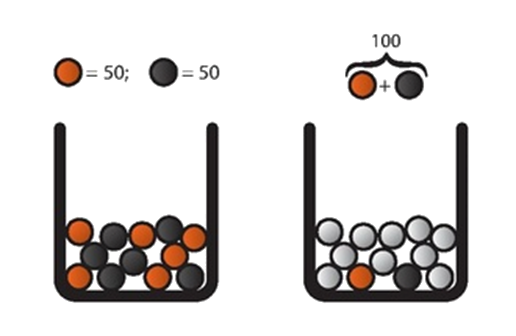
\includegraphics[width=0.4\textwidth]{img/Ellsberg-urn_alpha.png}
    \caption{The two Ellsberg urns: Urn 1 on the left contains well defined proportions of black and red balls, whereas for Urn 2 on the right the proportions are unknown.}
    \label{fig:Ellsberg}
\end{figure}

\strut

Subjects hold bets on the color of the balls to be drawn from the urns. A 
\emph{bet on black }``$b$'' yields $100$ Euro if the ball drawn from the urn
is black. Otherwise the payoff is zero. Similarly, \emph{betting on red }``$%
r$'', the subject earns $100$ Euro if a red ball is drawn and nothing
otherwise. Table~\ref{tab:Ellsberg} summarizes this choice problem.


\begin{table}[H]
\centering
\begin{tabular}{|l|c|c|c|c|}
\hline
& \multicolumn{2}{|c}{\emph{Urn 1}} & \multicolumn{2}{|c|}{\emph{Urn 2}} \\ 
\hline
& 50 & 50 & \multicolumn{2}{|c|}{100} \\ \hline
& \emph{Black} & \emph{Red} & \emph{Black} & \emph{Red} \\ \hline
$b$ (\emph{bet on black}) & $100$ & $0$ & $100$ & $0$ \\ \hline
$r$ (\emph{bet on red}) & $0$ & $100$ & $0$ & $100$ \\ \hline
\end{tabular}%
\caption{Payoff table (in Euros) for betting on \emph{black} or \emph{red} in the two urns.}
\label{tab:Ellsberg}
\end{table}


Holding a bet first on\emph{\ black} ($b$) and then on \emph{red }($r$),
subjects had to choose the urn on which they wanted to bet.

A large number of subjects, about 60 percent, choose to bet on the draw from
Urn 1 for both bets\footnote{%
The fact that subjects prefer to bet on the urn with the known proportion of
colors could be confirmed in many repetitions of the Ellsberg experiment. 
\cite{paper:AmbiguityReview} reviewed 39 experimental studies of the
Ellsberg experiments. They report a median number of 59 percent of ambiguity
averse subjects across all studies which they reviewed.}. These choices
clearly contradict the assumption that these subjects were maximizing subjective expected utility.

    
    \hfill --- Ellsberg's suggested thought experiment\footnote{The description has been borrowed from \cite{paper:EllsbergHilbert}, which is based on the original paper \cite{paper:Ellsberg1961}.}.
    \end{quote}





Empirical evidence has been gathered shortly in 1964 which supported ambiguity aversion\footnote{See \cite{paper:EmpiricalEllsbergBecker1964} and a more recent review citing several experimental results in \cite{paper:ExperimentalEllsbergReviewCamerer1992}.}

%{\it Psychological perspective:}
%\footnote{See \cite{paper:AmbiguityAndRationalityFrisch1988}.}

{\it Cognitive science of decision making:}
Brain studies show that humans might have dedicated brain areas involved in decision-making and accessing uncertain factors\footnote{For reference see \cite{thesis:NeuralDecisionMaking,paper:NeuroeconomicsOfDecisionMaking}.}.

{\it Ellsberge paradox and the proposed framework:}
At first glance -- with a naive and faulty application of the framework -- the Ellsberg paradox might seem natural. If the Agent imagines an adversarial player behind the uncertain (or ambiguous) factors, trying to prevent her from winning, then she will choose always the non-ambiguous urn. (In this thought process the Agent is assuming a zero-sum game, therefore she assumes that when she could bet on red, the ambiguous urn is full of black balls and full of red if she has the opportunity to bet on black.)

However if we faithfully follow the procedure suggested in the beginning of this essay, and the Agent assumes that the fictional player maximizes her regret instead of negative utility, then the effect vanishes. 
Lets examine the case, when the agent can bet on red balls. In this case if the trickster always provides an urn with full of black balls, then it can cause no regret. It created the worst situation, but the Agent can always choose the risky urn, therefore doing the best she can, without feeling any regret.
To cause regret, the trickster needs to give sometimes better then $50$-$50$ chances in the ambiguous urn. To maximize it’s objective the trickster will sometimes provide an urn full of red balls -- beside an urn full of black balls.
How often will the trickster choose a favourable composition? How the Agent is ought to play in equilibrium? The regret of choosing the ambiguous urn if it is full of back balls is $1/2 \ U(\text{``red''})+ 1/2 \ U(\text{``black''}) – \ U(\text{``black''}) = 1/2 \ U(\text{``red''})- 1/2 \ U(\text{``black''})$, and the regret of choosing the risky urn if the ambiguous urn is full of red balls is $U(\text{``red''}) - (1/2 \ U(\text{``red''})+ 1/2 \ U(\text{``black''})) = 1/2 \ U(\text{``red''})- 1/2 \ U(\text{``black''})$. (In all other cases the regret is zero, because the Agent could not have been making a better choice.) The two non-zero regrets are the same, therefore -- by realizing that for the Agent utility and negative regret differ only in an action-independent factor -- the game theoretical problem can be reduced to a simple Matching Pennies game. In which the equilibrium solution is choosing randomly for both players with 50\%-50\% chance (for the Agent choosing the risky urn with 50\%, and choosing the ambiguous urn with 50\%, while for the imaginary trickster choose an urn full of black balls with 50\% and fill the urn with red balls with 50\%).
The result remains the same if the Agent’s utility is not proportional to monetary gains, therefore in particular the Agent’s risk aversion is not changing this result.

There are variations of the dilemma and the thought process, however, which can alter the result.
The result may change in repeated scenarios if the Agent is risk averse i.e. (in frameworks compatible with expected utility theory) her utility function is concave.
If the number of repetitions goes to infinity, while keeping the maximum winnable amount to 100 Euros, then the dilemma now practically changes to an ``auction problem’’, where either we get 50 Euros, or gaining potentially 0 or 100 Euros with the ambiguous urn.
This changes the potential regrets as well, resulting a higher probability of choosing the risky urn for a risk averse Agent in equilibrium. This effect appears for small repetitions as well e.g. for two rounds. While this might explain some related phenomena such as ``home bias'' in finance\footnote{``Home bias is the tendency for investors to invest in stocks that are, literally, closer to home. For example, investors in most countries tend to invest heavily in stocks from their home country and very little in stocks from foreign countries.'' \cite{thesis:NeuralDecisionMaking}. For further references see \cite{paper:HomeBiasDisappearing,paper:HomeBias1991,paper:PuzzlesInMacroeconomics}.}, the same effect can be understood in the subjective expected utility theory with extreme priors (having more weight at the extreme ends of the ball distributions). Further, the construction of Ellsberg explicitly states that the choice is made once i.e. this is a one-shot decision problem.

We have to conclude that the Ellsberg paradox remains a paradox -- reflecting the framework's deeper compatibility with subjective expected utility theory --  however I believe this framework opens more avenues to understand the experimental results.  

\dots

\pgfornament[height=0.6cm]{72}

\paragraph{Allais paradox:}
\dots 

\pgfornament[height=0.6cm]{72}

\subsection*{Animal behaviour}

\paragraph{Advocating for compassion:}
I have to confess that I was reluctant to mention and cite the results of biological experiments because most of the time, I read the papers with feeling sorrow for the animals.
I convinced myself to write about the results found in these papers only because I might have a chance to promote the expansion of the circle of compassion\footnote{Circle of altruism is a similar concept in Peter Singer's book \cite{book:ExpandingCircle}, where he argues for the extension of ethics and morality by applying ``rationality''. 

Similar concepts, however, are compatible with various theological and philosophical frameworks. In the Neo-Confucian tradition an ``anthropocosmic'' vision emerged as the natural transcendence of egoism, parochialism, nationalism and anthropocentrism \cite{paper:TuWeimingNewConfucianHumanism}. 

In Indian religions (Hinduism, Buddhism and Jainism) animals are regarded as sentient beings \cite{book:EncyclopediaOfBuddhism} and their respect is derived from the central concept of ``ahimsa'' -- a principle of nonviolence \cite{britannica:Ahimsa}. 

Abrahamic religions view animals usually rather instrumentally. However, in the Judeo-Christian tradition if one interprets the scripture in Genesis not as ``rule over'' or ``have dominion over [\dots] animals'' but rather as stewardship and care, then the scripture is mostly compatible with a compassionate coexistence and cooperation with animals and non-human beings \cite{book:OnAnimalsInChristianity}. The folklore surrounding Francis of Assisi in Catholicism is a further testimony that a non-exploitative relationship -- at least in theory -- is compatible with this worldview. There are attempts to accommodate Islam to a more compassionate animal welfare as well \cite{paper:AnimalWelfareIslam}.

I do not try to indicate that all the mentioned worldviews imply compassion toward non-human beings, but it seems that effort has been made to accommodate them to a more inclusive view of being and coexistence. The driving force of this push might be an emergent tendency of our times. I may very well be under the spell of this prevailing sentiment, yet even after self-critical reflection I still believe this concern is worth addressing. 
}.
(My concern is not primarily focused on suffering -- although this makes the matter more painful to comprehend -- but the alienation of living beings, treating them as subjects or sometimes as objects\footnote{The objectification of animals can be spotted even at the language level. In contemporary English, farm animals appear more often in contexts similar to tools and raw materials then contexts referring to sentient beings i.e. people, wild animals or pets \cite{thesis:Anita}.}, and therefore preventing them from realizing their potential and engaging fully in the dance of life and being. I don't think that it is only harmful to ``them''; I believe it is harmful to us if we distance ourselves from the majority of living beings because the price for alienation -- and the capacity of being cruel -- is the feeling of isolation and boundedness. I am not advocating for treating animals and other living beings in the same way we treat humans. I promote practices which don't cause the evaporation of compassion and where animals are not viewed as subjects but as partners by whom we can engage and hopefully foster a mutually beneficial relationship. On the other hand, if we expand our circle of compassion to a broader range of living beings, then we enrich ourselves and can feel more connected and more at home in the world. Compassion and love are not getting less if given; it is just getting more.)

However, sadly, I can not point confidently to any institute or research center which I could promote as an example. This is partially because of my lack of first-hand experience and therefore the unreliability of my impressions about the circumstances in such facilities, but more importantly because in the present era we are so distant from a respectful compassionate and wise coexistence with other life forms and Nature as a whole that even the best examples might sound as cosmeticized cruelty from a more enlightened point of view.

To mention a few institutes, the \href{https://www.ab.mpg.de/}{Max Planck Institute of Animal Behavior} and the \href{https://janegoodall.org/}{Jane Goodall Institute} are hopefully setting a good example in high quality non-invasive, observational animal research. I might mention the Skylab\footnote{As an example a research paper elaborating on the method can be found here \cite{paper:SkyLabLin2024}.} concept in Center for the Evolutionary Origins of Human Behavior \href{https://www.ehub-kyoto-u.com/en}{EHUB} of Kyoto University in Japan where the participation in cognitive tests of chimpanzees is voluntary (rewarded by food), but overall the animals are still captive. A promising initiative for animal testing in biomedical studies has been proposed by providing \href{https://www.nytimes.com/2006/11/24/business/in-trials-for-new-cancer-drugs-family-pets-are-benefiting-too.html}{experimental oncological treatment} for dogs with cancer.

The list is of course not exhaustive and I am sure that I am not aware of many good examples. (And on the other hand I am not sure that there are no flaws and misconduct in the examples I gave.) But my point is not to judge or boycott institutes, but rather show that high quality research is possible with true mutualism between humans and animals\footnote{For example in \cite{paper:Domestication} domestication is defined in the following way: ``Domestication is a sustained multigenerational, mutualistic relationship in which one organism assumes a significant degree of influence over the reproduction and care of another
organism in order to secure a more predictable supply of a resource of interest, and through which the partner organism gains advantage over individuals that remain outside this relationship, thereby benefitting and often increasing the fitness of both the domesticator and the target domesticate.''}. My hope is that these examples pointing to a better direction can bring one step closer to a mindset shift, where humans recognize that they are in an unseparable unity with others life forms and the world and where instead of exploitation and conquering we will engage in cooperation.

\paragraph{Values of science and morality:}
In the previous paragraph I chose to advocate for a cause, but -- coming back to the main focus of the present essay -- it also serves as an example where ``scientific values'' can clash with personal moral values.
(Of course the problem can be framed as a question of separation and unity as well, but even in that case it shows that curiosity is sometimes in conflict with causing harm.)
It is a reminder that even ``scientific values'' should not be pushed to the extremes, and even for research usually a holistic approach is needed to balance between sometimes non-aligned values.

\paragraph{Ambiguity aversion in animals:}

There is empirical evidence showing that animals from several species show ambiguity aversion in laboratory settings.

However experimental results are reported mostly from non-human primates (apes and monkeys), suggesting that some cognitive similarity to humans is needed to observe such behaviour.


\begin{itemize}
    \item In non-human primates Ambiguity aversion has been observed\footnote{Decision-making of Capuchin monkeys \cite{thesis:AmbiguityAversionInCapuchinMonkeys}, Rhesus macaques \cite{paper:RhesusMacaquesAmbiguity}, Orangutans, Gorillas, Chimpanzees and Bonobos has been studied in \cite{paper:PrimatesAmbiguity} and \cite{paper:PrimateRandomArticle}. See also \cite{paper:ChimpanzeesBonobosAmbiguity}.};
    \item Studies found that several animals were able to find and act according to Nash equilibrium strategies in economic games\footnote{See a study focusing on non-human primates \cite{paper:EconomicGamesPrimates}. Rhesus monkeys randomize their choices according to Nash equilibrium, see \cite{paper:PrimateRandomArticle} for reference.}.
\end{itemize}

In the light of the previous paragraphs, my personal opinion is that in the area of economic behaviour no further experimental research is needed on captive animals. (While observational studies and more compassionatly/thoughtfully designed experiments could be illuminating.)

\dots

\pgfornament[height=0.6cm]{72}

\section*{Epilogue}

\dots

\pgfornament[height=0.6cm]{72}

{\centering
\vspace{1 cm}
  \Huge To be continued.\par


\begin{figure}[h]
    \centering
    \includegraphics[width=3cm]{img/Auryn.png}
\end{figure}

}




%To demonstrate, that such construction indeed provides ``reasonable'' decision making strategies, one has to explore and analyze the resulted strategies. This mainly mathematical task has been started by the fir

\newpage
\printbibliography

\end{document}
